\documentclass[a4paper,11pt]{article}
\pdfoutput=1 % if your are submitting a pdflatex (i.e. if you have
             % images in pdf, png or jpg format)

\usepackage{jcappub} % for details on the use of the package, please
                     % see the JCAP-author-manual

\usepackage[T1]{fontenc} % if needed


\usepackage{hyperref}
\usepackage{natbib}
\usepackage{subfiles}
\usepackage{aas_macros}
\usepackage{amsmath}
\usepackage{amssymb}
\usepackage{float}
% added for arxiv submission

\usepackage[section]{placeins}
\usepackage{graphicx}
% \usepackage{subcaption}
\usepackage{booktabs}
\usepackage[normalem]{ulem}
\usepackage{aas_macros}
\useunder{\uline}{\ul}{}


\usepackage{lettrine}
\input Zallman.fd
\renewcommand{\LettrineFontHook}{\usefont{U}{Zallman}{xl}{n}}
\LettrineTextFont{\itshape}
\setcounter{DefaultLines}{3}%

\newcommand{\unit}[1]{\ensuremath{\, \mathrm{#1}}}
\newcommand{\vbar}{\bar{v}}
\newcommand{\vesc}{v_{esc}}
\newcommand{\Rstar}{R_{\star}}
\newcommand{\Mstar}{M_{\star}}
\newcommand{\be}{\begin{equation}}
\newcommand{\ee}{\end{equation}}
\newcommand{\pn}{p_N(\tau)}
\newcommand{\Ncut}{N_{cut}}
\newcommand{\vn}{v_{N}}
\newcommand{\expmess}{\exp{\left(-\frac{3(\vn^2-\vesc^2)}{2\vbar^2}\right)}}

\title{\boldmath Dark Matter in Population III Stars}


\author{Ian K. Bania}
\author{(Advisor: Cosmin Ilie)}

\affiliation{Department of Physics and Astronomy, Colgate University\\
13 Oak Dr., Hamilton, NY 13346, U.S.A.}
 
% e-mail addresses: one for each author, in the same order as the authors
\emailAdd{ibania@colgate.edu}
\emailAdd{cilie@colgate.edu}

\journal{\text{Physics 492: Honors Thesis}}


\abstract{
    \\After scattering off nucleons, Dark matter (DM) particles may lose enough energy to become gravitationally bound to an astrophysical object.
    In order to become captured in this manner, super heavy DM may need to experience a number of successive scattering events.
    Once captured within a star, it is possible for DM to continue to upscatter off of nucleons and gain enough energy to escape the potential well in a process known as evaporation.
    In the case of captured self-annihilating DM it then becomes possible for heating from DM annihilations to be a significant source of energy production for Population III (Pop.~III) stars. 
    By implementing recently developed formalism of multiscatter capture in the stellar evolution code \texttt{MESA}, I model how Pop.~III stars react to heating from captured DM.
    Furthermore I use \texttt{MESA} models to calculate DM temperatures and evaporation rates in regions of interest.
    Next, I present early results on the influence DM heating has on stellar structure and evolution.
    Finally I explore whether or not \texttt{MESA} models of DM powered stars may be used to place competitive bounds on important DM properties.}


\begin{document}
\maketitle
% \flushbottom


% \pagenumbering{gobble}
\begin{section}{Motivating Dark Matter}
    %%% Galaxy Clusters %%%
    \lettrine{I}{n} 1933, while studying the velocity dispersion of galaxies in the Coma Cluster, Fritz Zwicky used redshift data to calculate that the radial velocities of the component galaxies varied by up to 2000 km/s \cite{Zwicky:1933}.
    Based on approximations of the cluster's mass made with a standard mass-luminosity relation, Zwicky calculated via the virial theorem an expected velocity dispersion of only 80 km/s, a value more than an order of magnitude less then the observed dispersion.

    Zwicky realized that, for the cluster to be gravitationally stable, it and its component galaxies must be far larger than originally implied by mass to light ratios.
    This was the first substantiative piece of observational evidence for the existence of Dark matter (DM), a class of material which we now know accounts for $\sim$85\% of the matter in the universe \cite{Bertone:2018}.

    While Zwicky and his contemporaries were quick to identify this discrepancy as being indicative of some previously unaccounted for source of mass, to early researchers `Dark matter' was an umbrella term for a variety of possible non-luminous or dim baryonic phenomena.
    In the three decades after Zwicky's initial work was published many others followed in his footsteps \cite{Zwicky:1937}\cite{Schwarzschild:1954}\cite{Babcock:1939}\cite{Kahn:1959}, making similar measurements of other galaxy clusters and nearby galaxies with many arriving at puzzling results: the inferred mass to light ratios, measured via mechanical observations of these objects, were consistently far greater than astronomers could easily explain.
     
    %%% Galactic Rotation Curves %%%
    Around the same time as Zwicky's work on the Coma Cluster, an equally troubling and perplexing open question in astrophysics was beginning to form.
    The stage was set in 1914 when Max Wolf and Vesto Slipher discovered that the spiral galaxy Andromeda rotates around its central core \cite{Wolf:1914}.
    However, it wasn't until 1970 when Vera Rubin and Kent Ford published their rotation curves of Andromeda \cite{Rubin:1970} that astrophysicists realized that a similar discrepancy could be observed in the outer regions of spiral galaxies.

    Where Rubin and Ford expected to see the rotational velocity slow with larger radii, they instead observed roughly constant velocities out to distances of $\sim$24 kpc.
    The nearly flat rotation curve, observed both in visible starlight and 21 cm hydrogen emission out to radii far beyond the visible disk, implied the existence of an enormous amount of non-luminous mass. 
    By 1980, flat rotation curves had been measured for dozens of other galaxies, adding to the considerable body of evidence supporting the notion that a significant fraction of the mass in galaxies was unaccounted for in existing mass-luminosity relations.

    %%% Gravitational Lensing %%%
    Another foundational piece of evidence for the existence of Dark matter comes from gravitational lensing.
    General relativity allows astronomers to determine the mass of a wide range of objects by observing how a background source of light is distorted by an occulting foreground object. By measuring the degree to which the light is bent, it is possible to calculate to a high degree of precision the mass of the foreground object.
    Not only does gravitational lensing provide a means to measure the mass of galaxies and clusters without having to rely on redshift measurements of velocities, but it also allows for far greater granularity in determining the distribution of mass within an object.
    This is especially useful for measuring mass present in areas lacking luminous matter, such as the space between component galaxies of a cluster, or the outer regions of galaxies at extremely large radii.

    The results of lensing observations are twofold:
    First, they provide strong corroboration to the rotation curves of galaxies and the velocity dispersion measurements of clusters.
    Secondly, they reveal numerous insights into the nature and distribution of Dark matter.
    Namely, that galaxies contain even more Dark matter than previously assumed, and that this Dark matter likely extends far beyond the visible edge of the galaxy in a spheroidal distribution referred to as a `halo' \cite{Freese:2017dm}.
    Additionally, it has been shown that there are likely significant amounts of extragalactic Dark matter which form large scale structures on cosmological scales \cite{Freese:2017dm}.

    %%% Cosmic Microwave Background and Baryonic Acoustic Oscillations %%%
    More data corroborating the existence of Dark matter comes in the form of the Cosmic Microwave Background radiation (CMB).
    This light, observed in the microwave, was emitted when the universe was only 380,000 years old and had cooled enough for electrons and baryons to recombine.
    Recombination allowed photons trapped in the opaque primordial soup by Thompson scattering to decouple and travel unimpeded, until measured by our telescopes today \cite{Bertone:2018}.
    The relic light of the CMB retains information that cosmologists are able to use to make inferences about the conditions in the early universe. Namely, anisotropies, or small variations in local temperatures, are a signature of points of higher density around which matter could clump and large scale structure could form.
    The photons and baryons clumped in these local density variations experienced pressure oscillations around an equilibrium \cite{Eisenstein:2005}, and DM interacting only gravitationally settled to the center of the density variations.
    At the time of recombination and decoupling, the photons were no longer subjected to these oscillations, effectively freezing the scale and amplitude of the acoustic oscillations into the light of the CMB at 380,000 years.
    This is measurable in the form of acoustic peaks in the power spectrum of the CMB anisotropies. 
    Since we have Dark and baryonic matter driving the oscillations differently, the scale of these peaks is dependent on the various density parameters.
    Today we can see these anisotropies manifested in the large scale structure of our universe, in the form of density variations of normal matter at more recent redshifts, known as baryonic acoustic oscillations (BAO).
    Because of this, many consider the CMB to provide practically irrefutable support for the existence of Dark matter in our universe \cite{Freese:2017dm}.

    %%% Other Evidence for Dark Matter %%%
    Other strong evidence for Dark matter includes the ongoing merger of the Bullet Cluster, where lensing measurements show Dark matter halos `overshooting' and moving past the resulting conglomeration of baryonic matter, which is slowed by frictional effects \cite{Clowe:2004}.
    Using gravitational weak lensing, and the Sunyaev–Zeldovich effect (i.e.~the inverse Compton scattering CMB photons by hot gas in clusters) astronomers can map both the distribution of DM and hot gas in the cluster, which provides a clear example of the non-electromagnetically interacting nature of Dark matter.
    Even further evidence comes in the form of the large scale structure we see in the universe today.
    Numerical simulations consistently show that without a large component of Dark matter, it would have been impossible for the galaxies and clusters we see today to have evolved in only 14 Gyr \cite{Springel:2005}.
    Dark matter halos in the early universe provided a `cosmic scaffolding' around which protogalaxies and the first generations of stars could coalesce. 

    In an attempt to motivate the following research and impress upon the reader its importance,  I have summarized some of the most significant pieces of evidence supporting the existence of Dark matter, however this treatment is far from exhaustive.
    Additional support comes from the Lambda Cold Dark Matter model ($\Lambda$CDM), the relative elemental abundances produced during Big Bang Nucleosynthesis, and the presence of hot gas in the outer reaches of galaxy clusters. 
    $\Lambda$CDM requires the existence of a significant amount of Dark matter to balance out dark energy and provide a topologically flat universe for us to exist in.
    During the first 20 minutes of the universe, temperatures were high enough in order to fuse baryons into deuterium, helium, and lithium.
    This process is known as Big Bang Nucleosynthesis, and in order for models to accurately predict the abundances cosmologists observe, baryonic matter is limited to comprising only 5\% of the mass-energy of the universe \cite{Coc:2004}.
\end{section}



\begin{section}{Dark Matter Particle Physics}
    As long as astronomers have known about the existence of Dark matter they have attempted to account for it with a variety of dim baryonic phenomena.
    In the early 20th century, when Dark matter only represented some limited discrepancies in the mass-luminosity ratios of large objects, many astronomers proposed a more rigorous accounting of cold gas and dust. 
    Despite numerous attempts to provide a baryonic theory of Dark matter, by the 1970s it was apparent that astronomers were not any closer to accounting for the missing mass, while new observations were indicating that Dark matter was far more abundant than previously thought. 

    Some more contemporary attempts at explanations of Dark matter which avoid non-baryonic particles are Massive Astrophysical Compact Halo Objects (MACHOs) and Modified Newtonian Dynamics (MOND).
    MACHOs are a hypothetical class of objects ranging from rogue exoplanets to dim white dwarfs which are proposed to account for Dark matter measured in galaxies and clusters \cite{Bertone:2018}.
    While these objects certainly exist in some quantity, attempts to observe them in large enough abundances have been unsuccessful.
    MOND postulates that the standard Newtonian picture is not accurate for tiny accelerations on galactic scales, and attempts to modify Newtonian mechanics in such a manner as to explain the numerous observed phenomena \cite{Bertone:2018}.
    While MOND has found limited success and is far from a consensus theory, it cannot be entirely disregarded at this time.

    Since the 1980s the leading class of Dark matter candidates have been non-baryonic `exotic' particles, with numerous specific candidate particles proposed. 
    Particle Dark matter is expected to be produced in the early universe before thermal decoupling and freeze out.
    That is to say, at high temperatures and number densities there is expected to be a process for converting standard model (SM) particles to DM and DM to SM.
    This two way process will be in an equilibrium as dictated by the temperature, but as the universe expands and number densities decrease, reaction rates will fall and soon the reaction will cease to occur on a cosmological scale.
    It is at this point that particle relic density is said to `freeze out'.
    If the temperature of the particle at the time of freeze out is much greater than the mass of the particle (in natural units that is), then we refer to these particles as hot thermal relics.
    If the converse is true, and the temperature is much smaller than the mass, then we have a cold thermal relic.

    A good example of the relativistic thermal relics are SM neutrinos, which have a freeze out temperature on the order of $\sim 1$ MeV, much greater then their mass \cite{Profumo}.
    In this sense neutrinos can be thought of as `hot Dark matter' but obviously they do not account for nearly enough of the universe's rest mass-energy budget to fit the bill for a DM particle.
    In general, we can talk about the particle interaction rate, $\Gamma$, as
    \begin{equation}
        \Gamma = n\sigma v,
    \end{equation}
    or when considering a class of particle with a distribution of temperatures we can use a thermal average:
    \begin{equation}
        \Gamma = n\langle\sigma v\rangle.
    \end{equation}
    Here, $\sigma$ is the cross section of the process responsible for DM production and $v$ is the relative velocity of the interaction.
    If we consider a cold DM particle, the condition of non-relativistic freeze will require that
    \begin{equation}
        n_{f.o.} \sim \frac{T_{f.o.}^{2}}{M_{P} ~ \sigma},
        \label{nfo}
    \end{equation}
    and the equilibrium number density $n$ will scale like
    \begin{equation}
        n \sim\left(m_{\chi} T\right)^{3 / 2} \exp \left(-\frac{m_{\chi}}{T}\right).
        \label{neqfo}
    \end{equation}
    Here $M_p$ is the reduced Planck mass, $m_\chi$ is DM mass and $T_{f.o.}$ denotes freeze out temperature.
    By applying Eq. \ref{nfo} and \ref{neqfo} we see
    \begin{equation}
        \sqrt{\frac{m_\chi}{T}} \cdot \exp\left[\frac{-m_\chi}{T}\right]=\frac{1}{m_{\chi} ~ M_{p} ~ \sigma},
    \end{equation}
    and since we are considering a cold particle by definition $\frac{m_\chi}{T} \gg 1$.
    By plugging a range of DM masses and cross sections that one would expect of a particle which interacts electro-weakly, we find that
    \begin{equation}
        20 \lesssim \frac{m_\chi}{T_{f.o.}} \lesssim 50.
    \end{equation}
    If we then consider that the Dark matter density parameter can be written in terms of the freeze out condition
    \begin{equation}
        \Omega_\chi = \frac{T_0^3}{\rho_c ~ M_p ~ \sigma ~T_{f.o.}},
    \end{equation}
    where $T_0$ is the temperature today, and $\rho_c$ is the critical density of the universe.
    By plugging in our constants and known cosmological parameters so that
    \begin{equation}
        \left(\frac{\Omega_{\chi}}{0.2}\right) \simeq \frac{m_\chi }{20~ T_{f.o.}}\left(\frac{10^{-8} \mathrm{GeV}^{-2}}{\sigma}\right),
    \end{equation}
    we find that a DM density parameter of $\Omega_\chi = 0.2$ produces a self-annihilation cross section of $\langle\sigma v\rangle \approx 3\times 10^{-26}$ cm$^3$ s$^{-1}$ \cite{Profumo}.
    This number is often referred to as the `WIMP miracle' because it corresponds to the same scale as one would expect from a particle with $m_\chi \simeq 10^2$ GeV that interacts electro-weakly.
    Furthermore $\Omega_\chi = 0.2$ is what we observe for the Dark matter component of the universe. 
    This class of particle, known as Weakly Interacting Massive Particles (WIMPs), was the favorite DM candidate particle up until fairly recently.

    One appealing feature of many WIMPs particles is how they arise organically from various theories in particle physics.
    Among the most prominent WIMP candidate particles are: the lightest supersymmetric particle implied by supersymmetry (SUSY), the Kaluza-Klein particle implied by a universal extra dimension (UED), or the lightest T-odd particle implied by little Higgs models.
    WIMPs will most likely have masses in the range of $10^9$ to $10^{12}$ eV \cite{Freese:2017dm}.

    Another promising particle candidate is the axion.
    The theoretical framework for axions arises from the strong-CP problem in particle physics independent of the astrophysical need for a Dark matter particle.
    Considerable work has already been performed in the pursuit of constraining the axion's mass \cite{Freese:2017dm}. If their mass is shown to lie between $10^{-3}$ and $10^{-6}$ eV, the axion may be a good Dark matter candidate \cite{Wilczek:1978}\cite{Weinberg:1978}. 
    Besides WIMPs and axions, other proposed Dark matter candidates include super massive WIMPs known as WIMPzillas \cite{Kolb:1999}, self interacting DM (SIDM) \cite{Carlson:1992}, strongly interacting massive particles (SIMPs) \cite{Hochberg:2014} \cite{Smirnov:2020}, and asymmetric DM \cite{Freese:2017dm}.

    Different DM models entail different methods of production and annihilation \cite{Ilie:2020popiii}, but the most common are p and s-wave annihilations where
    \begin{equation}
        \chi + \chi \to \text{SM} + \text{SM},
    \end{equation}
    SIMP annihilation \cite{Hochberg:2014} where
    \begin{equation}
        \chi + \chi  + \chi \to \chi + \chi ,
    \end{equation}
    and CoSIMP annihilation \cite{Smirnov:2020} where
    \begin{equation}
        \chi + \chi + \text{SM} \to \chi + \text{SM}.
    \end{equation}
    For this work I only consider $2 ~\chi \to 2$ SM annihilations , but it should be fairly simple to extend my methods to other annihilation models. 
\end{section}



\begin{section}{Direct Detection Efforts}
    %%% MOST RECENT EXPERIMENTAL BOUNDS FIG HERE ???
    \begin{figure}
        \centering
        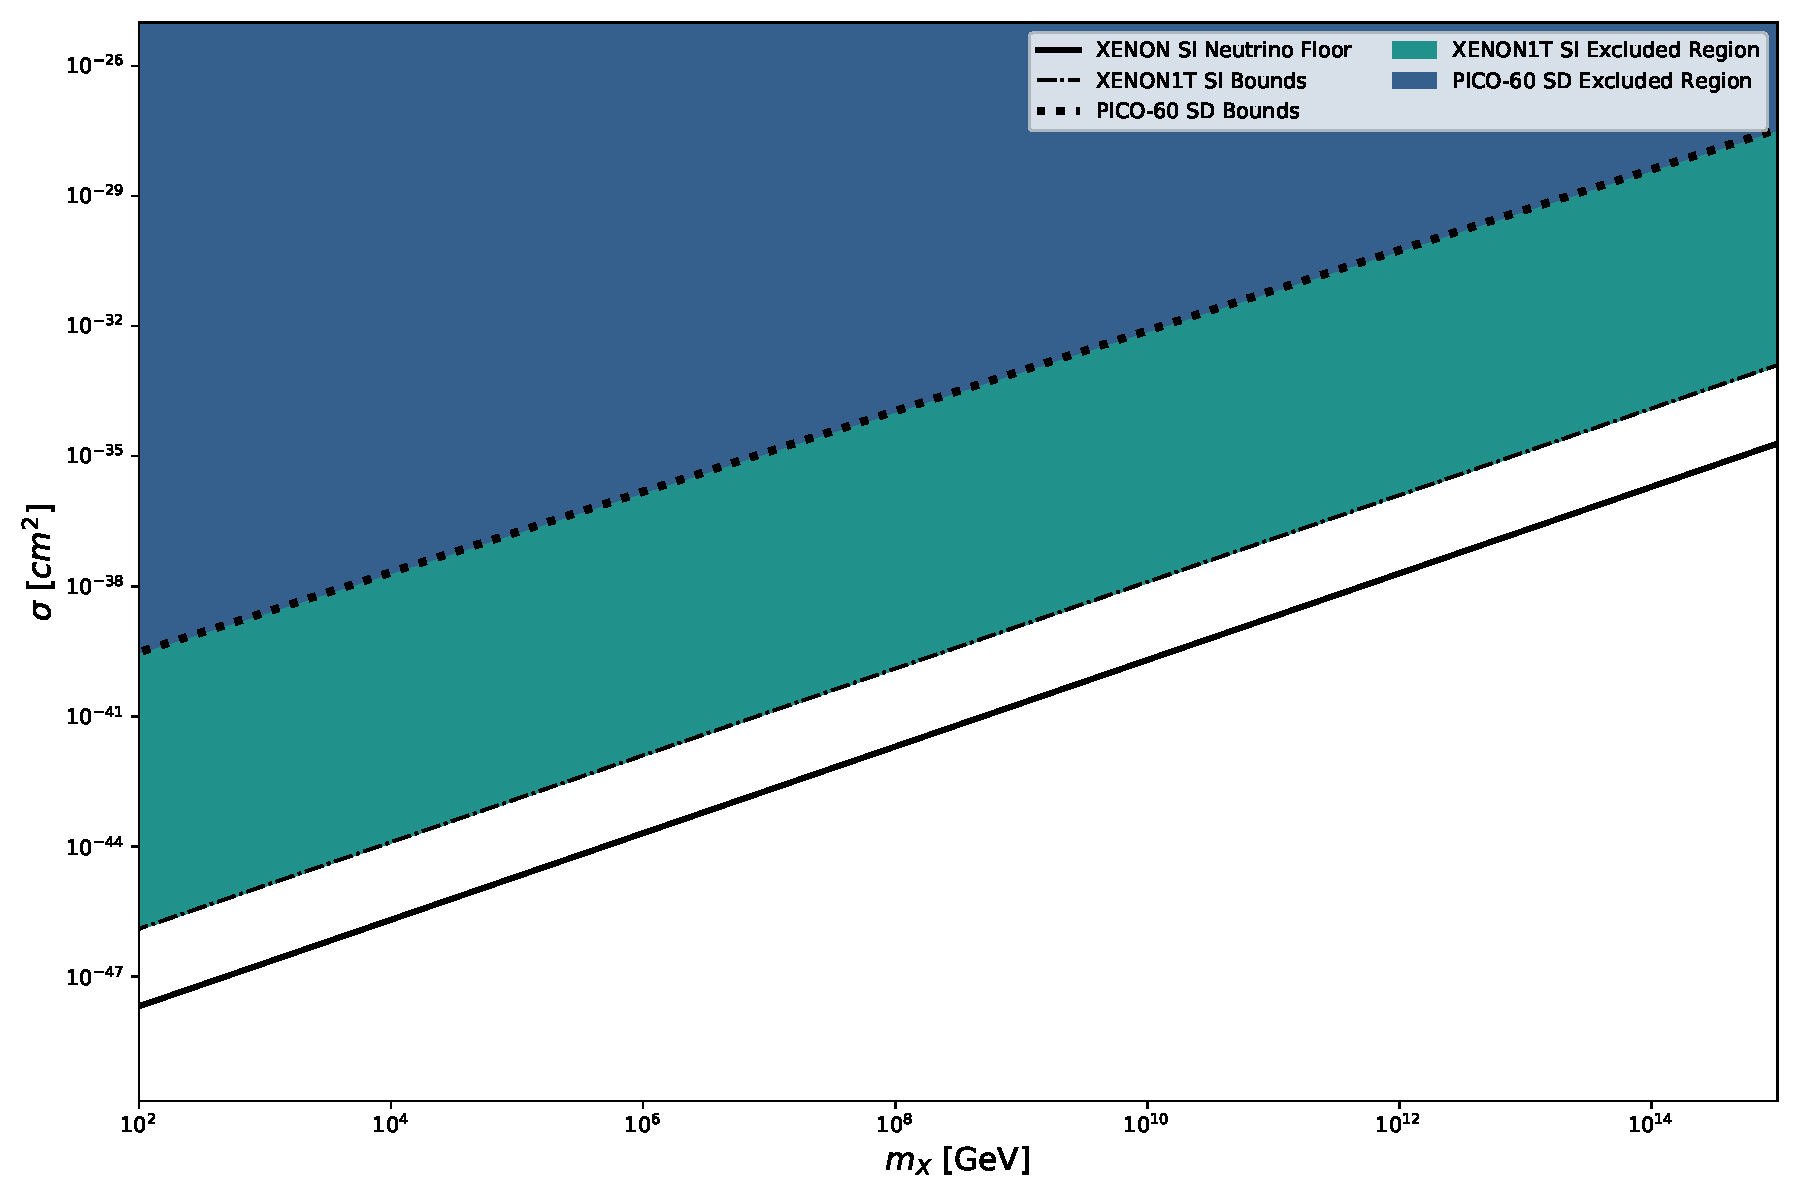
\includegraphics[width=0.9\textwidth]{bounds.pdf}
        \caption{Spin dependent (SD) and Spin Independent (SI) exclusion bounds on the $\sigma$\--$m_\chi$ parameter space from the PICO-60 and XENON1T direct detection experiments.}
        \label{bounds}
    \end{figure}
    %%% Direct Detection Experiments %%%
    Since the mid 1980s, astronomers and particle physicists alike have concerned themselves with detection of the particle responsible for the majority of the Dark matter in the universe.
    As the most favored DM candidates, WIMPs and axions have been the most sought after in direct detection, indirect detection and collider production experiments.
    For WIMPs specifically, there have been a dozen or so attempts at direct detection with many more in progress at time of writing.
    As a consequence of Earth's positioning in the Milky Way's Dark matter halo, we expect to see an annual modulation in detection events as we move into and out of the WIMP `wind' caused by the Sun's galactocentric motion \cite{Drunkier:1986}.
    The actual mechanism of WIMP detection comes down to measuring the energy deposited by a transiting WIMP as it collides with detection materials such as cryogenic germanium crystals or a heavy noble gas.
    As can be seen in \cite{Drunkier:1986} and \cite{Freese:2013}, the DM-nucleon cross section, i.e.~the probability of a WIMP scattering off one of the atomic nuclei in the detector, will scale with the atomic mass squared with
    \begin{equation}
        \sigma_{\mathrm{SI}}=\frac{4}{\pi} \mu^{2}\left[Z f_{\mathrm{p}}+(A-Z) f_{\mathrm{n}}\right]^{2},
    \end{equation}
    for spin-independent scattering, and
    \begin{equation}
        \sigma_{\mathrm{SD}}=\frac{32 \mu^{2}}{\pi} G_{F}^{2} J(J+1) \left( \frac{1}{J}\left(a_{\mathrm{p}}\left\langle S_{\mathrm{p}}\right\rangle+a_{\mathrm{n}}\left\langle S_{\mathrm{n}}\right\rangle\right)\right)^{2},
    \end{equation}
    for spin-dependent.
    Here $\mu$ is the WIMP-nucleus reduced mass, $Z$ is the number of protons in the nucleus, $A$ is the number of total nucleons, $G_F$ is the Fermi constant, and $J$ is the total spin of the nucleus.
    $\langle S_{\mathrm{P}}\rangle$ and $\langle S_{\mathrm{n}}\rangle$ are the averaged spin contributions from protons and neutrons, where $f_p$, $f_n$, $a_p$ and $a_n$ are effective couplings to protons and neutrons.
    This scaling is the motivation for the use of atoms with heavy and inert nuclei in Dark matter detection experiments.

    Another practical concern when detecting WIMPs are background counts from cosmic rays.
    The expected WIMP modulation signal pales in comparison to the noise of cosmic rays.
    Accordingly, detectors are located deep underground as a means of shielding, often in decommissioned mines.
    Despite this, a WIMP detection has remained elusive with all but one detector providing no statistically significant signal, and often excluding regions of the cross section-mass parameter space from the presence of a WIMP particle.
    The Italian program, originally  DAMA/NaI and now in its latest iteration DAMA/LIBRA, is the only detector that has claimed to have detected WIMPs \cite{Bernabei:2008} \cite{Bernabei:2018}.
    DAMA, a crystal scintillator detector built out of NaI, has collected 10 years of statistically distinct modulation, either from a 10 GeV or an 80 GeV WIMP.
    This is in apparent conflict with the null results from other non-NaI detectors worldwide, as well as the COSINE-100 detector, the only other apparatus besides DAMA using NaI crystals for detection.
    The preliminary COSINE-100 results, published in 2018 and 2019, have yet to show evidence supporting the modulation signal claimed by DAMA, but also remain inconclusive about its validity until the detector can reach the necessary precision levels, hopefully within the next two years \cite{Cosine:2018} \cite{Cosine:2019}.
    Other notable experiments that have done considerable work to constrain the spin-independent parameter space are the XENON, CDMS, and LUX projects.

    Other methods of WIMP detection involve probing the Dark matter parameter space via the use of single nucleons as target material, or by particle generation via high energy colliders such as the LHC at CERN.
    The net result of attempts at direct detection in the last 20 years are that the existence of a WIMP such as that predicted by supersymmetry theory or universal extra dimensions seems increasingly unlikely.
    This situation is only worsened by the fact that as particle physicists increase the sensitivities of their detectors to lower and lower cross sections, they approach the neutrino floor, a sensitivity at which any WIMP signal will become indistinguishable as detectors are lit up with background counts from neutrinos.
    The short comings of direct detection have prompted astronomers to think about alternative ways to constrain the properties of Dark matter, either via indirect detection of gamma rays produced by Dark matter annihilations in the galactic core (or nearby dwarf spheroidal satellite galaxies) or by measuring astrophysical properties of objects heated or influenced by Dark matter as proposed in  \cite{Ilie:2020popiii}, \cite{Leane:2021}, \cite{Ilie:2019} and \cite{Ilie:2020floor}.
\end{section}



\begin{section}{Modules for Experiments in Stellar Astrophysics (\texttt{MESA})}
    In order to fully assess the effects that DM heating may have on a complex astrophysical object such as a star, it becomes necessary to consider the effects that additional heating from DM will have over the course of an object's lifetime.
    To do this for Pop.~III stars, I use \texttt{MESA}, a 1-dimensional, stellar evolution package that combines the modeling of basic stellar structure equations with a variety of modular packages used to provide equations of state, opacity, nuclear reaction rates, elemental diffusion, stellar atmosphere conditions, surface pulsations, radiative transfer rates, ionization data and mixing lengths \cite{MESA:2011} \cite{MESA:2019}.
    \texttt{MESA} is written in Fortran 95 and supports OpenMP multi threaded parallelization.

    \texttt{MESA} and its component modules are controlled by `inlist' files, which contain hundreds of parameters used to control and simulate stars.
    \texttt{MESA} can build pre-main sequence models from scratch, or can be started from previously created models at any point during a stars evolutionary life span.
    To simulate the relevant physics in a reasonable amount of time, \texttt{MESA} dynamically adjusts its spatial and temporal resolution in order to optimize for compute times while also numerically solving the equations of stellar structure to the prescribed degree of accuracy.
    \texttt{MESA} models typically have hundreds to thousands of radial cells, and throughout a star's lifetime the timestep will vary from seconds to hundreds of thousands of years.

    In addition to its robust support for modeling a wide variety of stars in a range of physical scenarios, \texttt{MESA} also allows for the relatively painless addition of user-written code via the \texttt{run\_star\_extras.f} routine.
    This provides public interfaces that the user can use to alter or augment \texttt{MESA}'s built in calculations for mixing lengths, wind schemes, variable accretion rates, energy production rates, or a variety of other parameters.

    \texttt{MESA} provides users the option of beginning runs by either forming a ``pre-main sequence'' (pre-MS) model or beginning computation from a pre-calculated, user supplied, numerically stable model.
    Once this model is either generated or read in from a data file, \texttt{MESA star} will begin its computation in earnest.
    The formation process of the pre-MS model does not necessarily represent anything physical, and instead involves adding successive shells of mass and altering the composition of an internal starting model until it arrives at a star which meets the user specified initial conditions.
    Once this model is achieved, a number of `relax' timesteps are carried out where the model runs with no requirement for convergence.
    The naming of the pre-MS models can sometimes be misleading as the finished results of these models do not necessarily represent an object at Zero Age Main Sequence (ZAMS). The user may supply a number or arbitrary stopping conditions which halt the generation of the pre-MS model before ZAMS is reached.
    In fact, as we will see later, it is possible to simulate objects with \texttt{MESA} which have no true Zero Age Main Sequence. 

    % Relevant \texttt{MESA} parameters for this work will be related to mixing length theory and superadiabatic gradients, low metalicity opacities, 
\end{section}



\begin{section}{Multiscatter Capture Formalism}
    In 1987 Andrew Gould showed that in the case of single scattering, the DM capture rate of an astrophysical object can be described analytically \cite{Gould:1987}.
    Recently, in 2017, Joseph Bramante et al.~extended this formalism to encompass single component, multiscatter capture. 
    This formalism was laid out in \cite{Bramante:2017} and necessary corrections to it were presented in \cite{Ilie:2020Comment}.
    In this section I will outline their and others work on the topic.

    Let us consider the transit of a DM particle through a gravitationally bound object such as a star.
    We can approximate the average length of a trajectory through a star as twice its radius, $R_{*}$.
    Thus, as the DM particle passes through a star comprised of targets with a number density $n_T$, we can roughly describe the average number of scattering events as: 
    \begin{equation}
    N \approx 2 R_{*} n_T \sigma_T,
    \end{equation}
    where $\sigma_T$ is the scattering cross section between DM and the target particle \cite{Bramante:2017}.
    $N$ is a convenient parameter as it is useful in differentiating between the single and multiscatter regimes, and if we are only considering scattering off of hydrogen nuclei we can define the optical depth $\tau \equiv 2R_{*} \sigma n_p$.
    Where $\tau << 1$, single scattering formalism may be applied, however, in the regime where $\tau >> 1$, we must use the following multiscattering formulation.

    The first step in defining a multiscatter capture rate, wherein DM particles may undergo multiple scattering events before their velocity is reduced below the star's escape velocity, will be to analytically describe a partial capture rate $C_N$ after exactly $N$ collisions. Following \cite{Bramante:2017}, the partial capture rate can be schematically described as:
    $$ C_N = [\text{capture area}] \times [\text{DM flux}] \times [\text{prob. of N collisions}] \times [\text{prob. of capture on N$^{th}$ collision}]. $$
    Treating each of these terms in sequence, we turn our attention to the capture area, or the cross sectional area the star presents to a transiting DM particle, i.e.~$\pi R_*^2$.

    Next, we consider the DM flux and as in \cite{Bramante:2017} I will assume a Maxwell-Boltzmann distribution for the inherent velocities of the DM particles in the locality of the star.
    We will define the parameter $u$ as the velocity of the DM particle when it is at an arbitrarily far distance from the star, free from its gravitational influence.
    This distribution can be expressed as a number density of particles for which velocities fall in the range of $u$ to $u+du$:
    \begin{equation}
    f(u)du = 3\sqrt{\frac{6}{\pi}} \frac{n_{\chi}u^2}{\vbar^3} e^{-3u^2/(2\vbar^2)},
    \end{equation}
    where $\vbar$ is the dispersion velocity of the DM halo, and $n_{\chi}$ is the number density of DM particles \cite{Bramante:2017}.
    Making the assumption that the star has no relative velocity with respect to the DM halo (a reasonable approximation for Pop.~III stars), and that the halo has some arbitrarily large escape velocity, we can write the DM flux as:
    \begin{equation}
    F(n_{\chi}, u) =n_{\chi} \int_{0}^{\infty} \frac{f(u)du}{u} (u^2 + v^2_{esc}),
    \end{equation}
    where $v_{esc}$ is the escape velocity of the star.

    Now we turn our attention to third term $p_N(\tau)$, which describes the probability that a DM particle will undergo exactly N scattering events.
    We can use a Poisson distribution to describe this probability which integrates over all possible scattering angles, $\alpha$
    \begin{equation}
        p_N(\tau) = \frac{2}{N!}\int_{0}^{1} ae^{-\alpha \tau} (\alpha \tau )^N d\alpha = \frac{2}{\tau^2}\Big(N + 1 - \frac{\Gamma(N + 2, \tau)}{N!} \Big).
        \label{pnt}
    \end{equation}
    This integral can be analytically solved as done in \cite{Bramante:2017} \cite{Ilie:2019}. Here, $\Gamma(s,x)$ represents the upper incomplete gamma function as defined by
    \begin{equation}
        \Gamma(s,x) \equiv \int^\infty_x t^{s-1} e^{-t} dt .
    \end{equation}

    Finally, we treat the fourth term in $C_N$, $g_N(u)$ which describes the probability a DM particle will be captured by its $N$th scattering event.
    For clarity, this is \textbf{not} the probability that a DM particle will experience $N$ scattering events, and then be captured, but instead the probability of capture in the situation that it has undergone $N$ scatters. 
    If we consider a DM particle's kinetic energy, both prior to and after a scattering event, we can write the possible range of fractional energy loss from a scattering event depending on the angles of incidence:
    \begin{equation}
    0 \leq \frac{\Delta E_i}{E_i} \leq \beta_+,
    \end{equation}
    where $\beta_+$ is the maximum fractional energy loss and we define it as $\beta_+ \equiv 4m_p m_{\chi}/(m_{\chi} + m_p)^2$. 
    Furthermore, by defining the maximum velocity a DM particle can have while still being captured as:
    \begin{equation}
    u_{max;N} \equiv v_{esc} \sqrt{\Big(1- \frac{\beta_+}{2}\Big)^{-N} - 1},
    \end{equation}
    as is done in \cite{Bramante:2017}, we are then able to use $\Theta(x)$, the Heaviside step function, to express the desired probability as:
    \begin{equation}
    g_N(u) = \Theta(u_{max;N} - u).
    \end{equation}
    I.e.\text{ }when $u$ becomes less than $u_{max;N}$, there will be a capture probability of 1.

    %%% Capture rate plots
    \begin{figure}
        \centering
        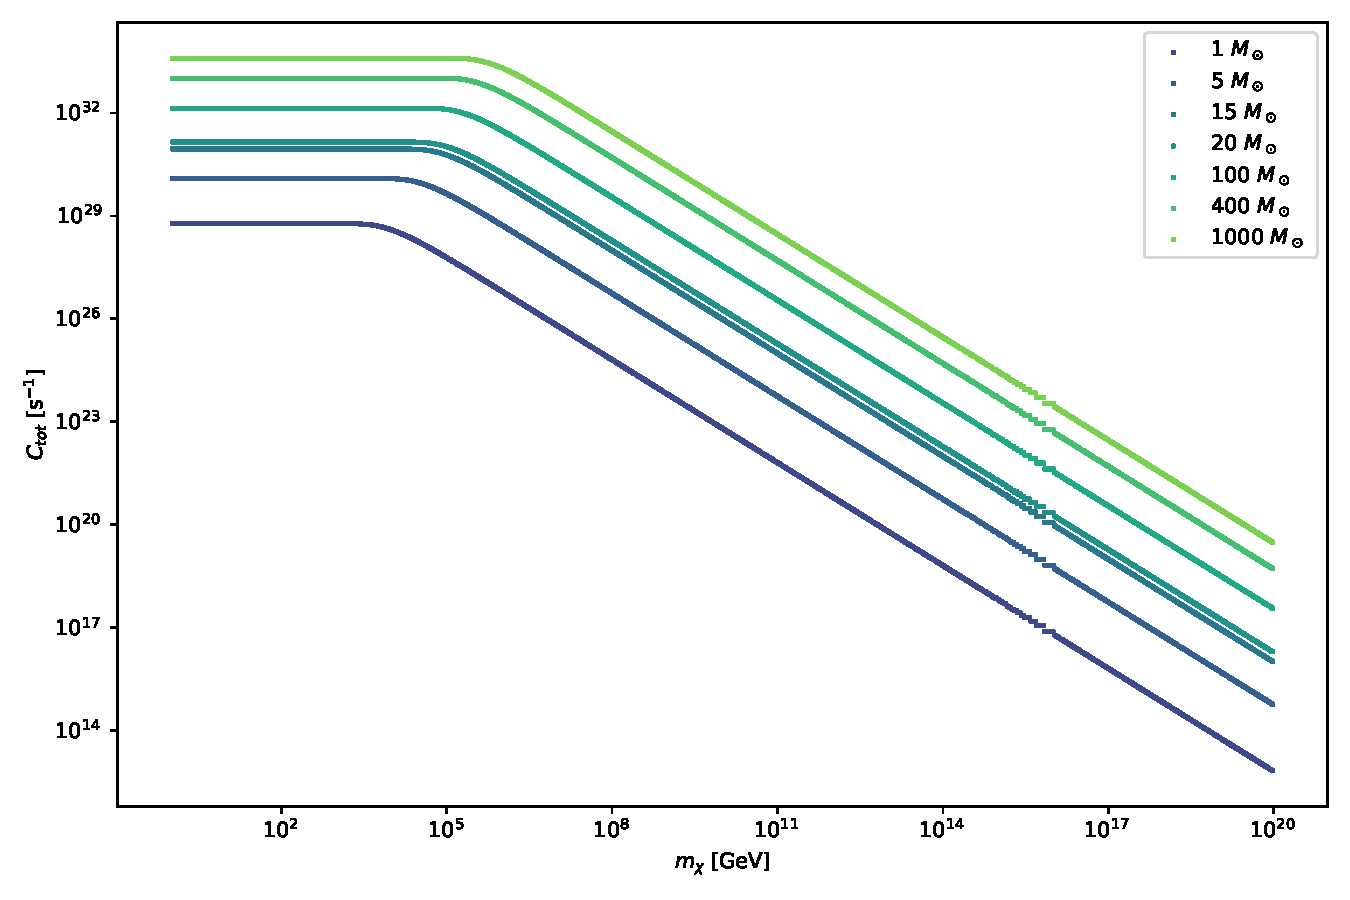
\includegraphics[width=0.9\textwidth]{Ctot1.pdf}
        \caption{DM capture rates of Pop.~III stars when $\rho_\chi = 10^{10}$ GeV cm$^{-3}$, $\bar{v} = 10^6$ cm s$^{-1}$, and $\sigma$ is calculated with the XENON1T bounds as seen in Fig. \ref{bounds}. These calculations were performed with the same Fortran 95 routine that is later embedded in \texttt{MESA} to calculate DM heating.}
    \end{figure}

    Combining the second and the fourth terms, it is now possible to express the total capture rate, $C_{tot}$, as an infinite sum across all of the partial capture rates:
    \begin{equation}
    %%%C_{tot} = \sum^{\infty}_{N=1} C_N = \sum^{\infty}_{N=1} \pi R^2_{*} \;\times\;  \frac{\rho_{\chi}}{m_{\chi}} \int_{0}^{\infty} \frac{f(u)du}{u} (u^2 + v^2_{esc}) \;\times\; p_N(\tau)  \;\times\;  g_N(u).
    C_{tot} = \sum_{N=1}^{\infty} C_{N} = \sum_{N=1}^{\infty} \underbrace{\pi R_*^2}_\textrm{capture area}\times \,\underbrace{\frac{\rho_X}{m_X} \int_0^{u_{max;N}} \dfrac{f(u)du}{u}\,(u^2+v_{ esc}^2)}_\textrm{flux of DM captured after $N$ collisions}\times \, \underbrace{p_{ N}(\tau).}_\textrm{prob. of $N$ collisions}
    \end{equation}
    Here $m_\chi$ and $\rho_\chi$ denote DM mass and DM density. 
    Following the work set forth in \cite{Bramante:2017}, the partial capture rate $C_N$ can be analytically simplified to:
    \begin{equation}
        C_N = \pi R_{*}^2 ~~ p_N(\tau)~~ \frac{\sqrt{6}\rho_{\chi}}{3\sqrt{\pi}\bar{v}m_{\chi}}\Bigg((2\bar{v}^2 + 3v_{esc}^2) - (2\bar{v}^2 + 3v_{N}^2) \exp\Big[\frac{-3(v_N^2 - v_{esc}^2)}{2\bar{v}^2} \Big]    \Bigg). 
        \label{eq22}
    \end{equation}
    While this formalism will hold for both single scatter and multiscatter regimes, if we plan on only considering the case where $\tau \gg 1$ (i.e.~the multiscatter regime) we can rewrite $C_N$ in an approximative fashion (see Eq. \ref{CN_aprox}).
    This will become especially useful later when we grapple with some of the issues inherent to numerically evaluating the capture rate.

    To summarize, DM particles transiting through an astrophysical object will scatter with the components of that object, here we consider nucleons.
    These scattering events may be modeled as kinematic collisions, and it is possible to express the energy the DM particles lose via these scatterings.
    Eventually, after enough scattering events a DM particle's velocity will be reduced to below the escape velocity of the star, effectively gravitationally capturing the DM in that star.
    In the next section, I will outline the process by which DM particles thermalize into a distribution around the center of a star and then self-annihilate to produce heat.
\end{section}



\begin{section}{Dark Matter Thermalization and Annihilation}
    Once a DM particle becomes gravitationally bound to a star, it will continue to scatter off baryonic nucleons and lose energy during its now orbital transits of the star. 
    This will lead the captured DM particles to thermalize into a distribution around the core of the star until the DM particle inevitably finds a partner to annihilate with.
    The relationship between the DM annihilation rate and the DM capture rate will be dictated by the timescale of thermalization.
    If this timescale for a given object is found to be comparatively short, it is possible to ignore it all together.
    In \cite{Freese:2008cap} the thermalization timescale is estimated to be
    \begin{equation}
    \tau_{th} \approx \frac{1}{\sigma~ v_{esc}~ n_p} \frac{m_{\chi}}{2 m_p},
    \end{equation}
    where we are only considering hydrogen nuclei as our target material so we use $n_p$ and $m_p$ as proton number density and mass.

    Due to this relatively short timescale as compared to a star's lifetime, and the small cross sections we are considering, we can assume the density of captured DM follows an isothermal distribution of uniform temperature $T_{\chi}$.
    In the case of larger DM-nucelon cross sections, one could consider the DM as being in local thermal equilibrium with the baryons of the star, $T_{\chi}(r) = T(r)$.
    The intermediate regime demands a more rigorous modeling of DM in a Maxwell-Boltzmann distribution.

    For the rest of this work, I only consider an isothermal DM distribution such as given in both \cite{Freese:2008cap} and \cite{Garani:2017}. So we have the number density of DM as
    \begin{equation}
        n_{\chi}(r) =  n_{c} e^{-m_{\chi} \Phi(r)/kT_c },
        \label{nchi}
    \end{equation}
    where $n_{c}$ is the number density of DM at the center of the star, $k$ is the Boltzmann constant, $T_c$ is the central temperature of the star, and $\Phi(r)$ is the gravitational potential as described by
    \begin{equation}
    \Phi(r) = \int_{0}^{r} \frac{GM(r)}{r^2} dr,
    \end{equation}
    Here $M(r)$ is the mass enclosed by a shell with radius $r$.
    Using this distribution of captured DM within the star, it then becomes possible to write the heating due to DM as such:
    \begin{equation}
        \int_{*} Q_{V} ~ dV  = f \times \Gamma_A \times 2 m_{\chi} ,
    \end{equation}
    where $f$ is the fraction of annihilation products that thermalize with the star (i.e.~electrons, and photons) as opposed to ones that escape the star without interaction (neutrinos). 

    For this work I take the arbitrary value of $f = 2/3$ as used in previous works \cite{Ilie:2019}.
    It is important to realize here that this is a model specific choice, and will depend on the specific DM candidate which we are considering. 
    Moreover, it should be noted that in outer regions of the star, if baryonic densities are low enough (such as they may be in the case of Dark stars) it is possible that some electrons and photons escape without fully thermalizing with the stellar gas.
    In \cite{Rindler-Daller:2020} it is shown that in principle, the assumption of $f = 2/3$ breaks down around $\sim 10^{-8}$ g cm$^{-3}$.
    However, in my models considering captured and not contracted DM, the entirety of the DM annihilation is occurring near the center of the star, and an assumption of $f=2/3$ (or whatever the fraction of non-neutrino by products we expect from our DM model) is appropriate. 

    Turning our attention to the relationship between the DM capture rate and the DM annihilation rate we can write the following differential equation as described in \cite{Ilie:2019}:
    \begin{equation}
        \dot{N}_\chi = C_{tot} - 2\Gamma_A 
        \label{diffeq}
    \end{equation}
    where $N$ is the number of DM particles captured within the star and $\Gamma_A$ is the DM annihilation rate.
    As we consider the effects of DM evaporation in the next section, we will see that this equation needs modification for DM masses below $m_\chi \simeq 10^2$ Gev.
    In \cite{Freese:2008cap} it is shown that for WIMPs in Pop.~III stars Eq.~\ref{diffeq} quickly reaches equilibrium as compared to the lifetime of the star. I make the assumption that it is safe to take
    \begin{equation}
        2\Gamma_A = C_{tot} 
        \label{rates}
    \end{equation}
    for the entirety of the star's lifetime, since in the models I consider we will only be overestimating the heating rate for the first few timesteps before equilibration is reached.
    Future iterations of this work will involve a calculation of the timescale of equilibration, $\tau_{eq}$, and incorporate that into the heating rate, but that is beyond the scope of this work.
\end{section}



\begin{section}{Evaporation of Captured Dark matter}
    \begin{figure}
        \centering
        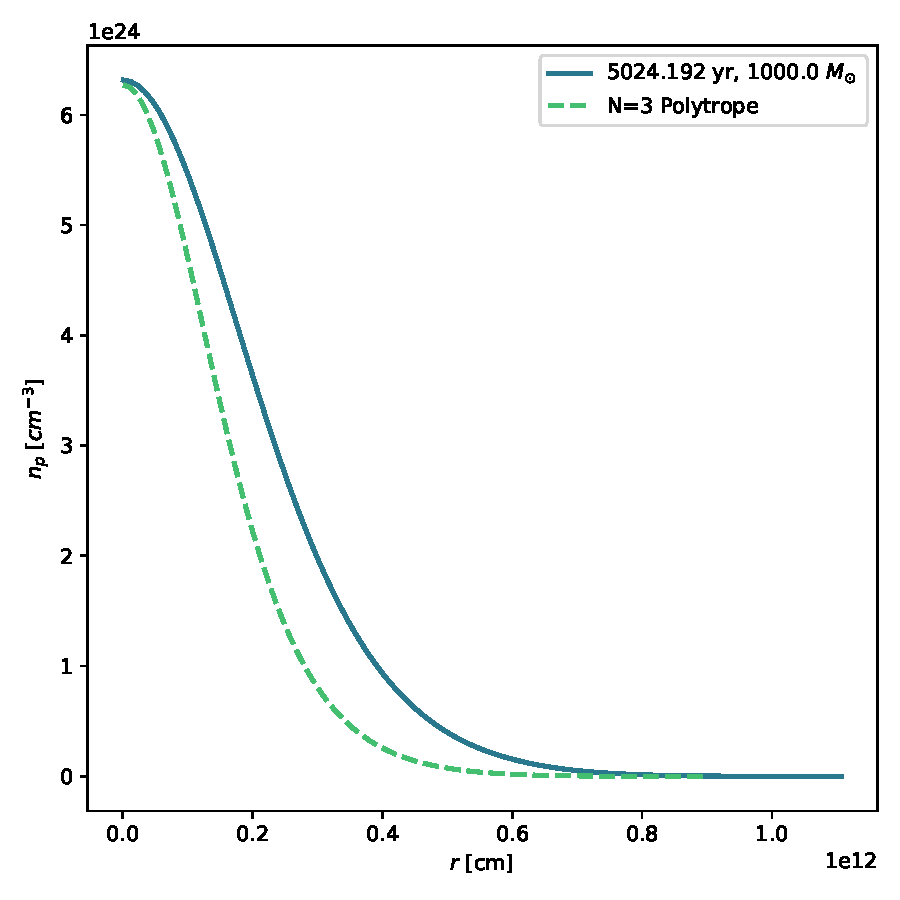
\includegraphics[width=0.49\textwidth]{np.pdf}
        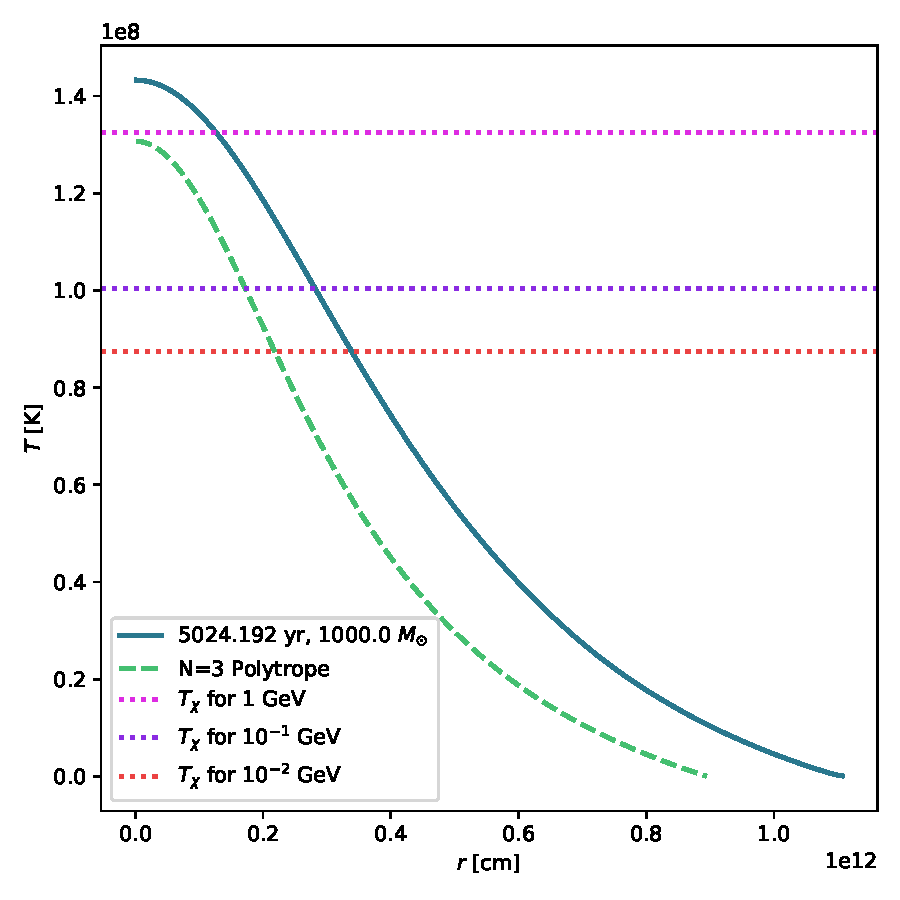
\includegraphics[width=0.49\textwidth]{Temp.pdf}
        \caption{Comparison between a 1000 $M_\odot$ Pop. III star from \texttt{MESA} and an $N=3$ polytrope.
        Hydrogen number density (left), and baryonic temperature (right).
        The DM temperatures ($T_\chi$) are calculated for the \texttt{MESA} star.}
        \label{MESAPOLY}
    \end{figure}
    Once captured DM has distributed itself isothermally within the star, at the same time it is undergoing the process of self annihilation it will continue to interact with the nuclei of star via the same method that captured it in the first place.
    The process of evaporation provides a competing effect to annihilation and must be factored into any calculations of DM heating made in regions where the evaporation is non-negligible.

    To calculate the temperature of this isothermal distribution we can use the volume integral put forth in \cite{Spergel:1985}
    \begin{equation}
        \int_0^{R_*} r^2 n_p(r) \bigg(\frac{m_p T_\chi + m_\chi T(r)}{m_x m_p} \bigg)^{1/2} (T(r) - T_\chi) \exp \Big[ \frac{-m_\chi \Phi(r)}{k T_\chi} \Big] dr = 0.
        \label{SP85}
    \end{equation}
    This is a statement of zero net heat flow between the baryons in the star and the captured DM particles.
    Essentially, lower temperature DM is able to gain energy, and higher temperature DM is able to lose it until the DM reaches an isothermal distribution.
    In \cite{Ilie:2020popiii}, values for DM temperature captured within a Pop.~III star are computed using an $N=3$ polytrope.
    To check that this approximation is appropriate, I model Pop.~III stars of 100 $M_{\odot}$, 300 $M_{\odot}$, and 1000 $M_{\odot}$ in \texttt{MESA} without DM heating.
    In order to correctly model large, radiation dominated stars with inefficient convective envelopes, I use the `MLT++' approach as described in \cite{MESA:2013}.
    This prevents a superadiabatic gradient from driving the model's timestep to computationally prohibitive small values.
    For other inlist values I look to \cite{Windhorst:2019} which provides a canonical example of modeling Pop. III stars in \texttt{MESA}.
    Notably, I chose an initial metalicity from big bang nucleosynthesis of $Z = 2 \times 10^{-16}$.
    The results of the \texttt{MESA} runs confirm that $N=3$ polytropes are good first order approximations of Pop.~III stars and selected radial profiles relevant to evaporation can be seen in Fig.~\ref{MESAPOLY}.
    
    For the calculation of $T_\chi$, I take radial data arrays from the stars at Zero Age Main Sequence (ZAMS) to use in equation Eq.~\ref{SP85}.
    I define ZAMS in this context be when $L_{nuc} \geq 0.9 ~ L_{tot}$.
    First I fit arbitrary interpolation functions to the temperature, mass density, hydrogen fraction, and gravitational acceleration arrays from \texttt{MESA}.
    I then proceed to define $T(r)$, $n_p(r)$ and $\Phi(r)$ in terms of those interpolations, and I numerically evaluate the integral in Eq.~\ref{SP85} using an initial guess of $T_\chi = T_c$.
    By using \texttt{SciPy}'s `\texttt{fsolve}' routine I solve for $T_\chi$ over a range of Dark matter masses: {$10^{-6} \to 10^4$ GeV} and while considering the stellar parameters derived from \texttt{MESA} runs of 100 $M_\odot$, 300 $M_\odot$, and 1000 $M_\odot$ Pop. III stars. 

    \begin{figure}
        \centering
        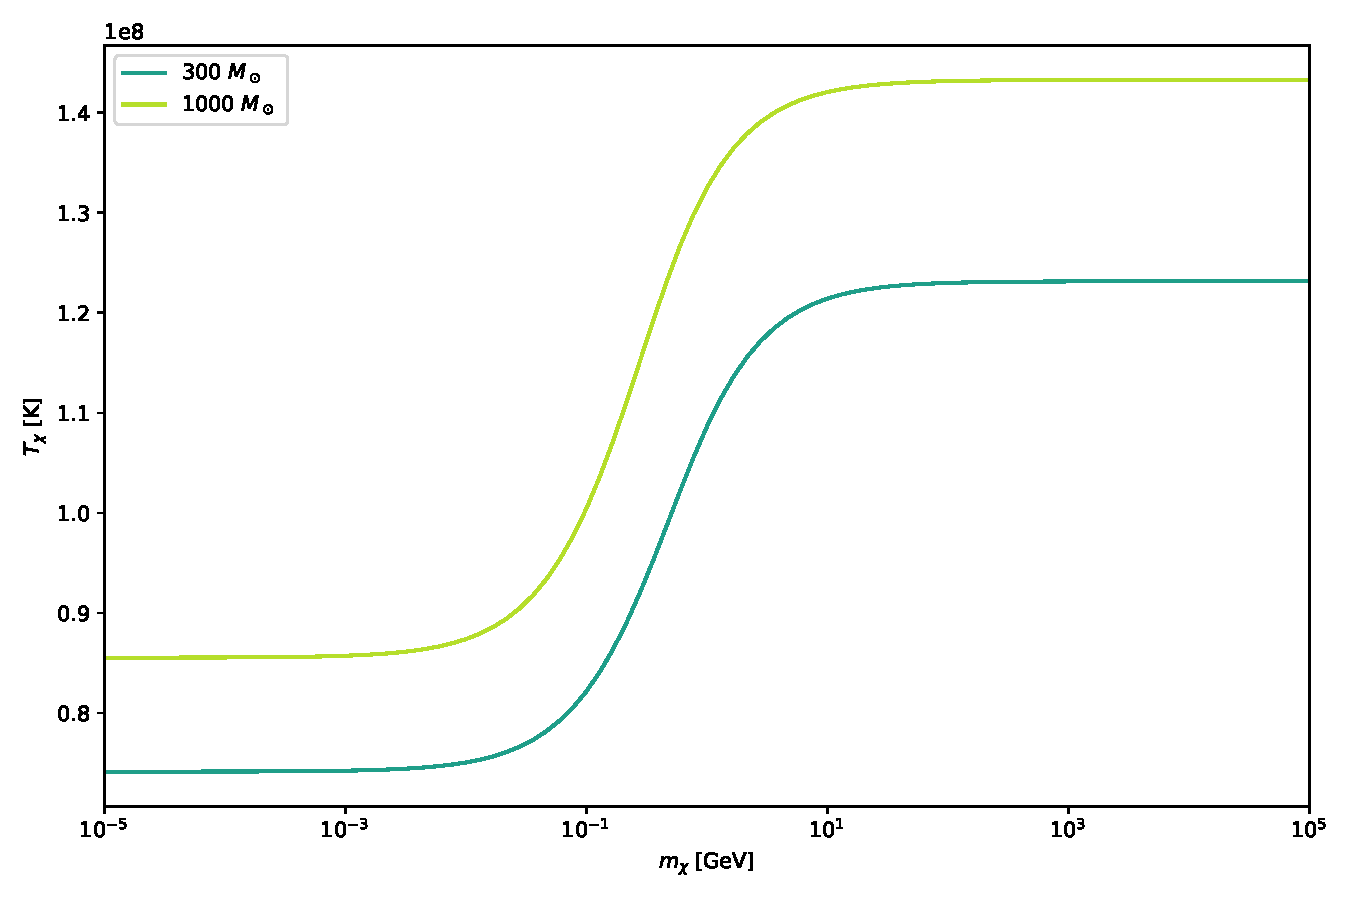
\includegraphics[width=0.9\textwidth]{Tchi.pdf}
        \caption{DM temperature as a function of DM mass, calculated for 300 $M_\odot$ and 1000 $M_\odot$ \texttt{MESA} models at ZAMS.}
    \end{figure}

    Using the temperature of the DM distribution we are now able to calculate an evaporation rate as a function of $m_\chi$.
    In Andrew Gould's 1987 paper on WIMPs in the Sun, he derives a closed analytical form for the evaporation rate for the shell evaporation rate $R(w|v)$ \cite{Gould:1987}. 
    To do this, Gould uses a truncated Maxwell-Boltzmann distribution which I reproduce here with the \textbf{correct} normalization factor as pointed out in \cite{Ilie:2020popiii}:
    \begin{equation}
        f(w) = \frac{\exp[-w^2 / v_\chi^2] ~ \Theta(v_c - w) }{\pi^{3/2} ~ v_\chi^3 \bigg(\text{erf}[v_c / v_\chi] - \frac{2 v_c}{\pi v_{\chi}} \exp[-v_c^2 / v_{\chi}^2 ] \bigg)}.
        \label{evapf}
    \end{equation}
    Here $w$ denotes DM speed and the average DM speed is $v_\chi \equiv \sqrt{2T_\chi/m_\chi}$.
    $v_c$ is the speed at which the distribution is truncated. For this work I take $v_c(r) = v_{esc}(r)$, that is to say, the cutoff speed at a certain radius is simply the escape velocity at that same radius.

    Gould goes on to derive a shell specific scattering rate, i.e.~the rate at which particles in a shell of radius $r$ up or down scatter from speed $w$ to speed $v$.
    Then, by integrating this over post-scattering velocity space, i.e.~$v$, from the cutoff speed ($v_{esc}$) to infinity, he produces an analytical expression for the rate at which particles with velocity $w$ in a specific shell escape the star.
    Finally, by integrating this and the distribution in Eq.~\ref{evapf} over pre-scattering velocity space $w$, he finds the evaporation rate of a specific shell.
    The general analytical form of this rate is
    \begin{multline}
        R(v_c|v_{esc}) = \frac{2}{\pi} \bigg(\frac{2T}{m_\chi}\bigg)^{1/2} \bigg(\frac{T}{T_\chi}\bigg)^{3/2} \sigma n_p n_\chi \\
        \Bigg[\exp\bigg[-\Big(\frac{\mu_+}{\xi}\Big)^2 \frac{E_e}{T_\chi}\bigg] \bigg( \frac{\mu\mu_-}{\nu\xi} \Big[\frac{\xi^2}{\nu} - \frac{\mu_+\mu_-}{\mu} \Big] + \frac{\mu_+^3}{\xi(\nu -\mu)}  \bigg) \chi(\gamma_-, \gamma_+) \\
        + \exp\Big[\frac{-E_c}{T_\chi}\Big] \frac{\mu}{\nu} \bigg(\alpha_+ \alpha_- - \frac{1}{2\mu} + \mu_-^2 \Big(\frac{1}{\mu} - \frac{1}{\nu}\Big) \bigg)\chi(\alpha_-, \alpha_+) \\ 
        - \exp\Big[\frac{-E_c}{T_\chi}\Big] \exp\Big[-\frac{E_e - E_c}{T}\Big] \frac{\mu_+^2}{\nu-\mu}\chi(\beta_-, \beta_+)      \\
        - \exp\Big[\frac{-E_c}{T_\chi} - \alpha_-^2\Big] \frac{\mu}{2\nu} \alpha_+ + \exp\Big[\frac{-E_c}{T_\chi} - \alpha_+^2\Big] \frac{\mu}{2\nu} \alpha_- \Bigg],
        \label{evapr}
    \end{multline}
    where the following definitions apply:
    \begin{equation*}
        \alpha_{\pm} \equiv \Big(\frac{m_p}{2T}\Big)^{1/2} (\mu_+ v_{esc} \pm \mu_- v_{c}) , 
    \end{equation*}
    \begin{equation*}
        \beta_{\pm} \equiv \Big(\frac{m_p}{2T}\Big)^{1/2} (\mu_- v_{esc} \pm \mu_+ v_{c}) ,
    \end{equation*}
    \begin{equation*}
        \gamma_{\pm} \equiv \Big(\frac{m_p}{2T}\Big)^{1/2} (\rho v_{esc} \pm \xi v_{c}) , 
    \end{equation*}
    \begin{equation*}
        \chi(a,b) \equiv \int^b_a e^{-y^2} dy = \frac{\sqrt{\pi}}{2} \Big(\text{erf}[b] - \text{erf}[a] \Big), 
    \end{equation*}
    \begin{equation*}
        \mu_{\pm} \equiv \frac{\mu \pm 1}{2} , 
    \end{equation*}
    \begin{equation*}
        E_e \equiv \frac{m_\chi v_{esc}^2}{2}, ~~~~~~ E_c \equiv \frac{m_\chi v_c^2}{2} ,
    \end{equation*}
    \begin{equation*}
        \xi^2 \equiv \mu_-^2 + \nu, ~~~~~~ \rho \equiv \frac{\mu_+\mu_-}{\xi} ,
    \end{equation*}
    \begin{equation*}
        \mu \equiv \frac{m_\chi}{m_p}, ~~~\text{and}~~~ \nu \equiv \mu \frac{T}{T_\chi} .
    \end{equation*}
    Also, note here that for brevity we write $T(r)$ as $T$, $v_{esc}(r)$ as $v_{esc}$ and $v_{c}(r)$ as $v_c$. The radial dependence is still there however, as the entire expression for $R(v_c | v_{esc})$ is shell specific.

    \begin{figure}
        \centering
        \includegraphics[width=0.9\textwidth]{Evap.pdf}
        \caption{DM evaporation coefficient computed for a 1000 $M_\odot$ star modeled with \texttt{MESA} (solid) and an $N=3$ polytrope (dotted). Here a value of $\sigma = 10^{-43}$ cm$^2$ was used.}
        \label{evap}
    \end{figure}

    It is with Eq.~\ref{evapr} that I can then calculate the total evaporation using \texttt{MESA} data files. 
    The final expression for the evaporation coefficient $E$ can be written in terms of a volume integral over the whole star
    \begin{equation}
        E = \frac{\int_0^{R_*} r^2~ n_\chi(r)~ R(v_c | v_{esc})~~ dV}{\int_0^{R_*} r^2~ n_\chi(r) ~~dV},
    \end{equation}
    where $n_\chi(r)$ is the same isothermal distribution we found in Eq.~\ref{nchi}. 
    Thus, the total evaporation rate for a star is $E N_\chi$ where $N_\chi$ is the total number of DM particles captured within the star.
    Using this, we may append Eq.~\ref{diffeq} to describe the relationship between capture, evaporation, and annihilation to write
    \begin{equation}
        \dot{N}_\chi = C_{tot} - 2\Gamma_A - E N_\chi.
        \label{newdiffeq}
    \end{equation}

    It can be seen from Fig.~\ref{evap} that any differences between \texttt{MESA} models and an $N=3$ polytrope have a negligible effect on evaporation rates. 
    Furthermore, it is clear that for Pop.~III stars, evaporation only comes into play for DM masses $m_\chi < 10^2$ GeV, well below the range of masses I will consider in this work. 
\end{section}



\begin{section}{Numerical Methods for Calculating DM Heating in \texttt{MESA}}
    In \texttt{MESA}, in order to augment energy produced via nuclear reactions with an additional source of heat like that from DM annihilations, one can use the \texttt{other\_energy\_implicit} hook.
    The arrays that must be calculated and set are listed in Table \ref{arrays}.
    \begin{table}
    \begin{center}
    \begin{tabular}{ |c|c| } 
     \hline
     \texttt{extra\_heat} & $Q_m$ \\ 
     \hline
     \texttt{d\_extra\_heat\_dlnR00} & $\frac{\partial Q_{m}(k)}{\partial \ln[r(k)]}$ \\ 
     \hline
     \texttt{d\_extra\_heat\_dlnRp1} & $\frac{\partial Q_{m}(k)}{\partial \ln[r(k+1)]}$ \\ 
     \hline
     \texttt{d\_extra\_heat\_dlndm1} & $\frac{\partial Q_{m}(k)}{\partial \ln[\rho(k-1)]}$  \\ 
     \hline
     \texttt{d\_extra\_heat\_dlnd00} & $\frac{\partial Q_{m}(k)}{\partial \ln[\rho(k)]}$  \\ 
     \hline
     \texttt{d\_extra\_heat\_dlndp1} & $\frac{\partial Q_{m}(k)}{\partial \ln[\rho(k+1)]}$  \\ 
     \hline
     \texttt{d\_extra\_heat\_dlnTm1} & $\frac{\partial Q_{m}(k)}{\partial \ln[T(k-1)]}$  \\ 
     \hline
     \texttt{d\_extra\_heat\_dlnT00} & $\frac{\partial Q_{m}(k)}{\partial \ln[T(k)]}$  \\ 
     \hline
     \texttt{d\_extra\_heat\_dlnTp1} & $\frac{\partial Q_{m}(k)}{\partial \ln[T(k+1)]}$  \\ 
     \hline
    \end{tabular}
    \caption{\texttt{MESA}'s `\texttt{other\_energy\_implicit}' arrays.}
    \label{arrays}
    \end{center}
    \end{table}

    The \texttt{extra\_heat} array takes the form of energy rate density, in the units of ergs s$^{-1}$ g$^{-1}$, whereas arrays ending with \texttt{lnR**} are partial derivatives with respect to radius, arrays ending with \texttt{lnd**} are partial derivatives with respect to baryonic density, and arrays ending with \texttt{lnT**} are partial derivatives with respect to temperature.
    The partial derivatives with \texttt{*m1} suffixes describe the change of the heating rate density with respect to the parameter of differentiation in the cell \textbf{above} the one where the heating rate density is evaluated, whereas the ones with \texttt{*p1} suffixes describe the change of the heating rate density with respect to the parameter of differentiation in the cell \textbf{below} the one where the heating rate density is evaluated.
    The variables suffixed with \texttt{*00} are simply standard partial derivatives.

    Therefore, for a given radial cell within \texttt{MESA} we can express the energy production rate due to DM annihilation as: 
    \begin{equation}
        \int_{cell} Q_{V} ~ dV = \frac{\int_{cell} r^2 ~n_{\chi}(r)^2~ dr}{\int_* r^2~ n_{\chi}(r)^2 ~dr} \times C_{tot} \times f \times m_{chi}
        \label{qm}
    \end{equation}
    By normalizing the captured DM distribution, we are provided with a fraction by which we can multiply the energy production rate for the whole star, while also avoiding calculating the central DM number density.
    Here $Q_V$ is the heating rate per unit volume, and $Q_m$ is the heating rate per unit mass.

    Finally, since \texttt{MESA}'s \texttt{extra\_heat} interface takes as input an array of energy rate mass density for all the cells in the star, we can express the energy production rate for a given cell per unit mass as follows: 
    \begin{equation}
        \frac{\int_{cell} Q_{V} ~ dV}{m_{cell}}  = \frac{\int_{cell} r^2 \exp[-2m_{\chi} \Phi(r) / kT_c]~dr}{\int_{*} r^2 \exp[-2m_{\chi} \Phi(r) / kT_c]~dr} \times \frac{C_{tot} f m_{\chi}}{m_{cell}}.
        \label{Qmpercell}
    \end{equation}
    As part of the \texttt{other\_energy\_implicit} hook, \texttt{MESA} also has inputs for partial derivatives of the \texttt{extra\_heat} profile, with respect to density, radius, and temperature. These allow for the fully self-consistent addition of heat to \texttt{MESA}.
    As described above, I calculate them numerically for use in the model.

    Unfortunately, since the captured DM distribution, and thus the DM heating rate, depend on enclosed baryonic mass, $M(r)$, which we read as an array from the model, we cannot take these partial derivatives analytically, and instead we must evaluate them numerically. 
    For a given cell $k$, I do this simply:
    \begin{equation}
        \texttt{d\_extra\_heat\_dlnT00} = \frac{\partial Q_{m}(k)}{\partial \ln[T(k)]} =
        \frac{Q_{m}(k+1) - Q_{m}(k-1)}{\ln[T(k+1)] - \ln[T(k-1)]} ,
    \end{equation}
    \begin{equation}
        \texttt{d\_extra\_heat\_dlnTp1} = \frac{\partial Q_{m}(k)}{\partial \ln[T(k+1)]} =
        \frac{Q_{m}(k+1) - Q_{m}(k-1)}{\ln[T(k+2)] - \ln[T(k)]} ,
    \end{equation}
    \begin{equation}
        \texttt{d\_extra\_heat\_dlnTm1} = \frac{\partial Q_{m}(k)}{\partial \ln[T(k-1)]} =
        \frac{Q_{m}(k+1) - Q_{m}(k-1)}{\ln[T(1)] - \ln[T(k-2)]}.
    \end{equation}
    The same is done with respect to $\ln(r)$ and $\ln(\rho)$.
    Edge cases for the two outermost and the two innermost cells of the star are approximated appropriately by taking partials centered on cell boundaries instead of cell centers.

    In order to accurately model Pop.~III stars, I adopt many of the same inlist parameters as used in \cite{Windhorst:2019}.
    Namely, I use the `gold' tolerances for \texttt{MESA}'s newton hydrodynamic solver, I take the same metalicity of $Z = 2 \times 10^{-16}$ as in the previous section, I use the `MLT++' version of mixing length theory as described previously, and I use a $\frac{dE}{dt}$ form of the energy conservation equation (as opposed to the $\frac{dL}{dm}$ version).
    Finally, I use the standard `dutch' wind scheme, with a scaling factor of 0.8 since here I am considering non-rotating stars.

    To assess the effects of DM heating on Pop.~III stars, I use two methods: I model the stellar evolution of a pre-main sequence star as it accretes mass from a surrounding minihalo, or I take a Pop.~III star at ZAMS with no continuing accretion.
    Both stars exist in a region of high DM density, and during each timestep I calculate additional heating from DM annihilations to be used in the newton solver.
    The model iterates on a given timestep, adjusting stellar parameters (and thus DM heating) until it reaches convergence.
    In order to do this, I make the assumptions discussed above: First, that the differential equation governing the relationship between capture and annihilations will reach equilibrium on a timescale much shorter than the star's lifetime.
    And second, that captured DM will quickly distribute itself along an isothermal density profile within the star.
    While I do calculate the number density profile each timestep, the density profile almost always falls entirely within the innermost radial cell of the star.
    The only exception is when running \texttt{MESA} with a manually increased number of grid points.

    With these assumptions made, in each timestep I proceed to read stellar characteristics from the \texttt{MESA} model. I sum the number of scatterings, $N$, across the partial capture rate as described by Eq.~\ref{eq22} to the cutoff point, $N_{cut}$.
    By statistically relating the point at which the total capture rate sum converges to the optical depth $\tau$, one can see that $N_{cut}$ equates roughly with $\tau$ as shown in \cite{Ilie:2019}.
    Previous numerical implementations of this capture sum involved a cutoff criterion based on the relative values of the most recently summed terms.
    However, in order to allow the sum to be written in a thread-safe manner and parallelized with the OpenMP interface, I use the cutoff criterion $N_{cut} = 2\tau$ as a means of preserving accuracy without incurring too much extra computational expense.
    For large $\tau$, being able to calculate the sum in a parallel manner on up to 32 threads (using Colgate University's Turing compute cluster) is invaluable in allowing \texttt{MESA} models to run in a reasonable amount of time.

    After the calculation of the capture rate for the entirety of the star, I then calculate the normalizing factor for the captured DM density profile via a numerical integral over the entire star.
    This can be seen as the denominator of Eq.~\ref{qm}.
    Next, to calculate the numerator of Eq.~\ref{qm}, I loop over each cell in the star, and numerically integrate the captured DM density profile from the bottom to the top of each radial cell.
    From here, I can evaluate Eq.~\ref{qm} in full for each cell in the star, providing the energy rate density on a cell-by-cell basis.
    Finally, using arrays of temperature and density read in from \texttt{MESA}, it is possible to take the numerical partial derivatives of each value in our \texttt{extra\_heat} array with respect to radius, density and temperature.

    It is important to note that when using 64-bit floating point variables to evaluate $p_N(\tau)$ at large values of $\tau$ one can encounter issues with arithmetic overflow.
    Since 170!~is the largest factorial capable of being stored by a 64-bit floating point, we are effectively limited to evaluating the sum of $C_N$, of which $p_N(\tau)$ is a term, at values of $\tau$ below 170.
    This issue can be curtailed using the approximate form
    \begin{equation}
        p_N(\tau)  \simeq \frac{2}{\tau^2} (N+1) \Theta(\tau - N),
    \end{equation}
    instead of Eq.~\ref{pnt} whenever $\tau \gg 1$ \cite{Ilie:2020popiii}.
    This form is derived from the right hand side of Eq.~\ref{pnt} by applying the definition of the gamma function.



    Another numerical issue is encountered when dealing with large values of $m_{\chi}$. 
    For most Pop. III stars, at DM masses above $10^{17}$ GeV there is a considerable loss-of-significance error from the subtraction of $v_N$ and $v_{esc}$ in the exponential term of Eq.~\ref{eq22}.
    To overcome this difficultly inherent in doing large number arithmetic with 64-bit variables, I use the following approximation put forth in \cite{Bramante:2017}:
    \begin{equation}
        C_N \simeq \sqrt{24 \pi}~ p_N(\tau) ~ G ~ \frac{\rho_{\chi}}{m_{\chi}} ~M_{*} R_{*} ~\frac{1}{\bar{v}}~ \Bigg(1 - \Big(1 + \frac{2A_N^2 \bar{v}^2}{3v_{esc}^2}\Big)\exp[-A_N^2] \Bigg), 
        \label{CN_aprox}
    \end{equation}
    where the approximation holds true for the limit that $v_{esc} \gg \bar{v}, m_{\chi} \gg m$, and $A_N^2$ is defined
    $$A_N^2 = \frac{3v_{esc}^2 N m_p}{\bar{v} m_{\chi}}.$$
    I use this approximative form when $m_{\chi} > 10^{16}$ GeV.
\end{section}



\begin{section}{Constraining the Properties of Dark matter}
    The stars we study, known as Population III stars, are the first stellar generation and are characterized by their extremely low metallicity.
    That is to say, Pop.~III stars are comprised entirely of hydrogen and helium.
    This is due to the fact that elements heavier than beryllium have yet to be fused in stellar cores and then distributed via super novae. 
    In previous work the assumption has been made that a star's total luminosity will be the sum from the DM contribution and nuclear burning. 
    This assumes there is no significant effect on nuclear reaction rates, stellar structure or evolution.
    In \cite{Ilie:2020popiii} it is shown that by making this assumption one can use the Eddington limit to place competitive bounds on the $(\rho_\chi \times \sigma)$ \--- $m_\chi$ parameter space.

    The Eddington limit is the maximum luminosity at which a star of a given mass can shine.
    Fundamentally this is a statement of hydrostatic equilibrium, as increasing the luminosity, and thus the outward radiation pressure, would drive super-Eddington winds, expelling material from the surface of the star until an equilibrium is once again reached.
    The Eddington limit can be expressed in terms of the gravitational constant $G$, opacity $\kappa$ and stellar mass $M_*$
    \begin{equation}
        L_{Edd} = \frac{4\pi G M_*}{\kappa},
        \label{edd}
    \end{equation}
    and thus in a simple model there is the following inequality:
    \begin{equation}
        L_{*} = L_{nuc} + L_\chi \leq \frac{4\pi G M_*}{\kappa}. 
        \label{ineq}
    \end{equation}
    From Eq.~\ref{qm} one can see that the total stellar heating, and thus luminosity from Dark matter, $L_\chi$, will be
    \begin{equation}
    L_\chi = \int_{*} Q_{V} ~ dV = C_{tot} \times f \times m_{chi}.
    \end{equation}
    Then, by calculating total capture rates via the method described in the previous section, one may use Eq.~\ref{ineq} to describe the maximum possible Pop. III mass for a given set of DM parameters. 

    If a Pop. III star is then observed to exist at a certain mass, by sweeping the parameter space with this inequality, one may place exclusion bounds similar to those created by direct detection experiments.
    More simply put: if a 500 $M_\odot$ star is seen to exist, then the areas of the DM parameter space where a 500 $M_\odot$ is greater than the maximum stellar mass allowed by the Eddington limit may be excluded.

    In this work I take a slightly more complex approach, I use \texttt{MESA} to model 78 different Pop. III stars, 72 which were augmented by DM heating, and 6 which were not augmented so they function as controls.
    I consider a range of stellar masses $M_*: \{100 \to 1000 M_\odot \}$, and DM parameters $\rho_\chi: \{10^{13} \to 10^{16}$ GeV cm$^{-3}\}$, $m_\chi: \{10^4 \to 10^{14}$ GeV $\}$, and $\sigma: \{10^{-46} \to 10^{-34}$ cm$^2\}$. 
    I explore a logarithmically spaced grid across $m_\chi$ and $\rho_\chi$, and I fix $\sigma$ to $m_\chi$ using the deepest exclusion bounds found from XENON1T:
    \begin{equation}
        \sigma  = 1.26 \times 10^{-40} \bigg(\frac{m_\chi}{10^8 \text{ GeV}}\bigg) \text{ cm}^2.
    \end{equation}
    In doing so, I find that instead of super-Eddington winds enforcing a maximum stellar mass, the DM heated stars I model are macroscopically very similar to my control Pop.~III stars.
    Regardless of the DM parameters tested, I see almost identical radii between the two classes of objects, very similar luminosities, and negligible rates of mass loss in both objects. 
    The only place where DM heated stars deviate from traditionally heated ones is at the star's core with its internal structure and composition.
    While these results are extremely counterintuitive, and may or may not represent an actual physical phenomenon, I will present them in the next section with the hope that further work may either discover the shortcoming in my numerical methods, or shed light on the process occurring here.
\end{section}



\begin{section}{The Effects of DM Heating on Stellar Structure and Evolution}
    \begin{figure}
        \centering
        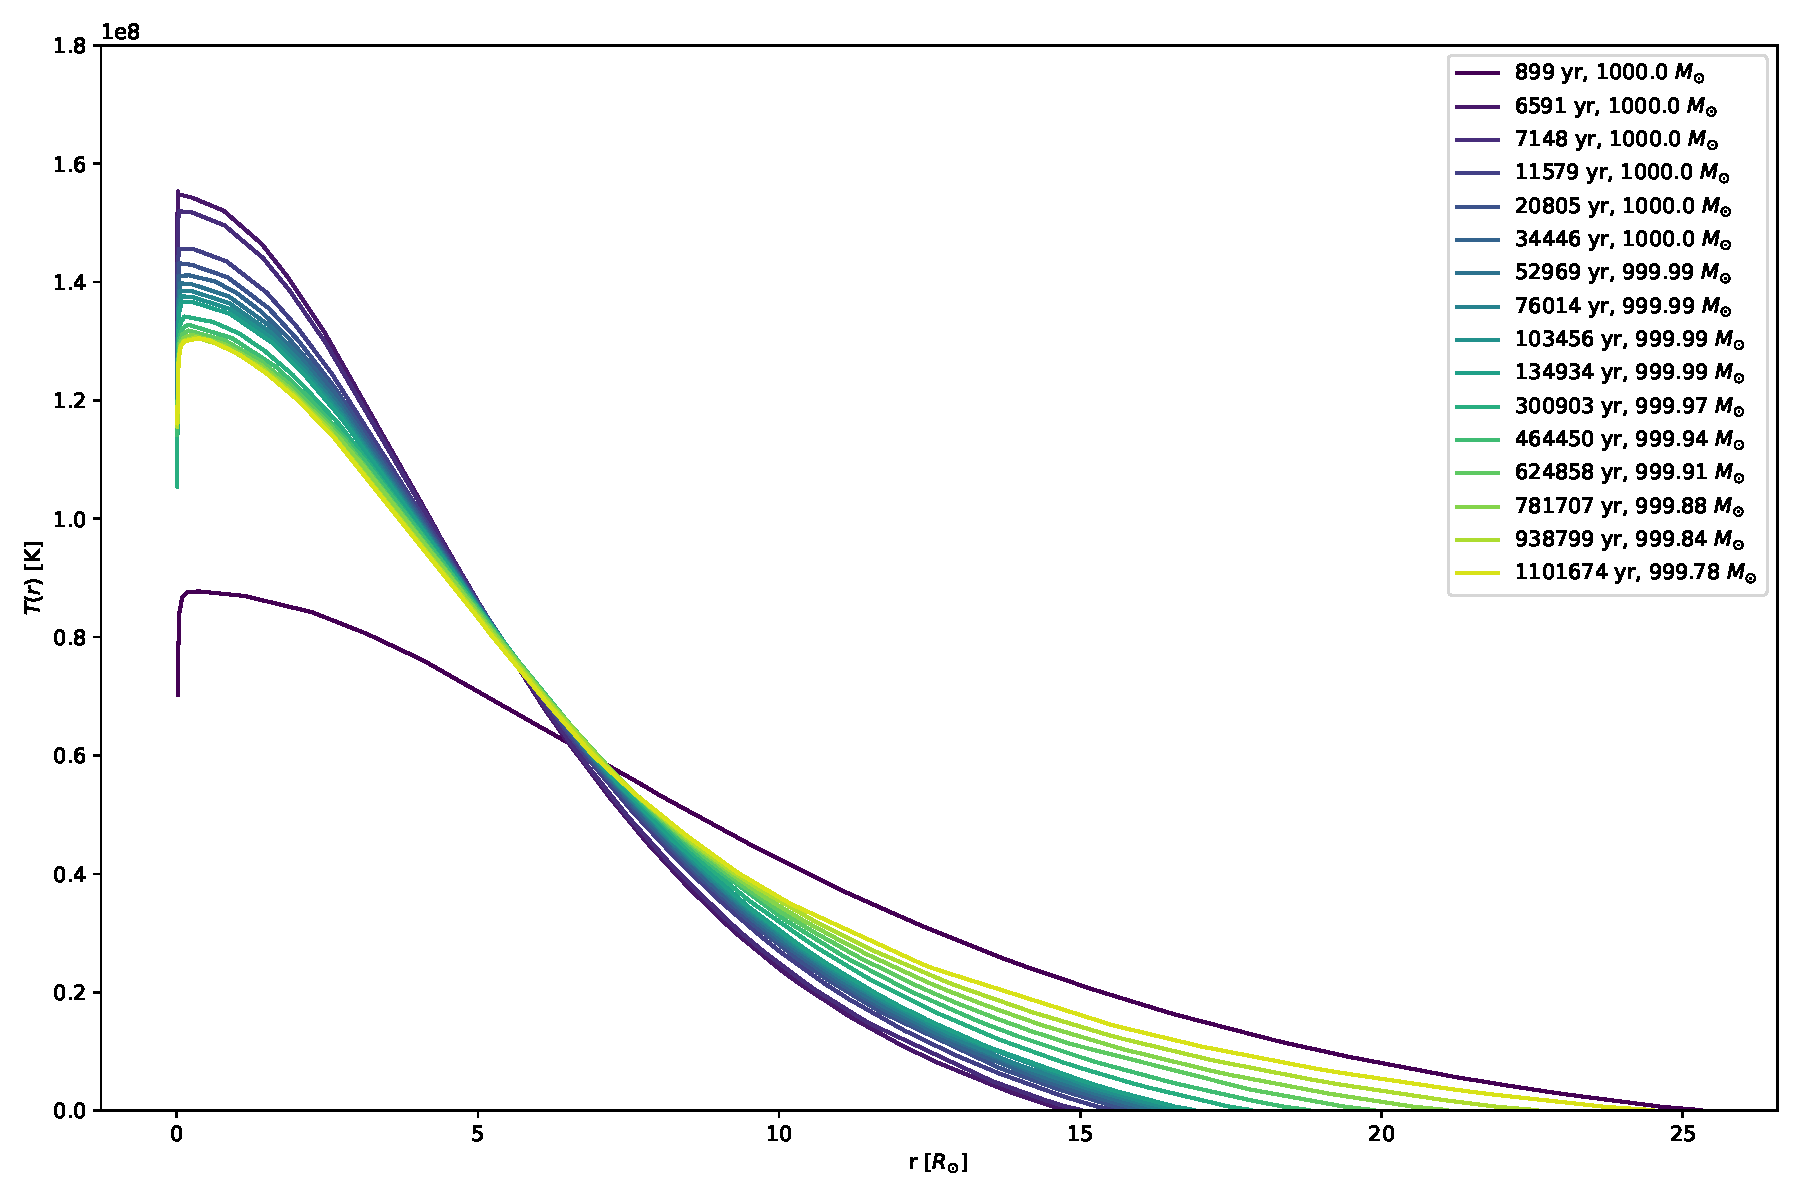
\includegraphics[width=0.49\textwidth]{T_profile_DM.pdf}
        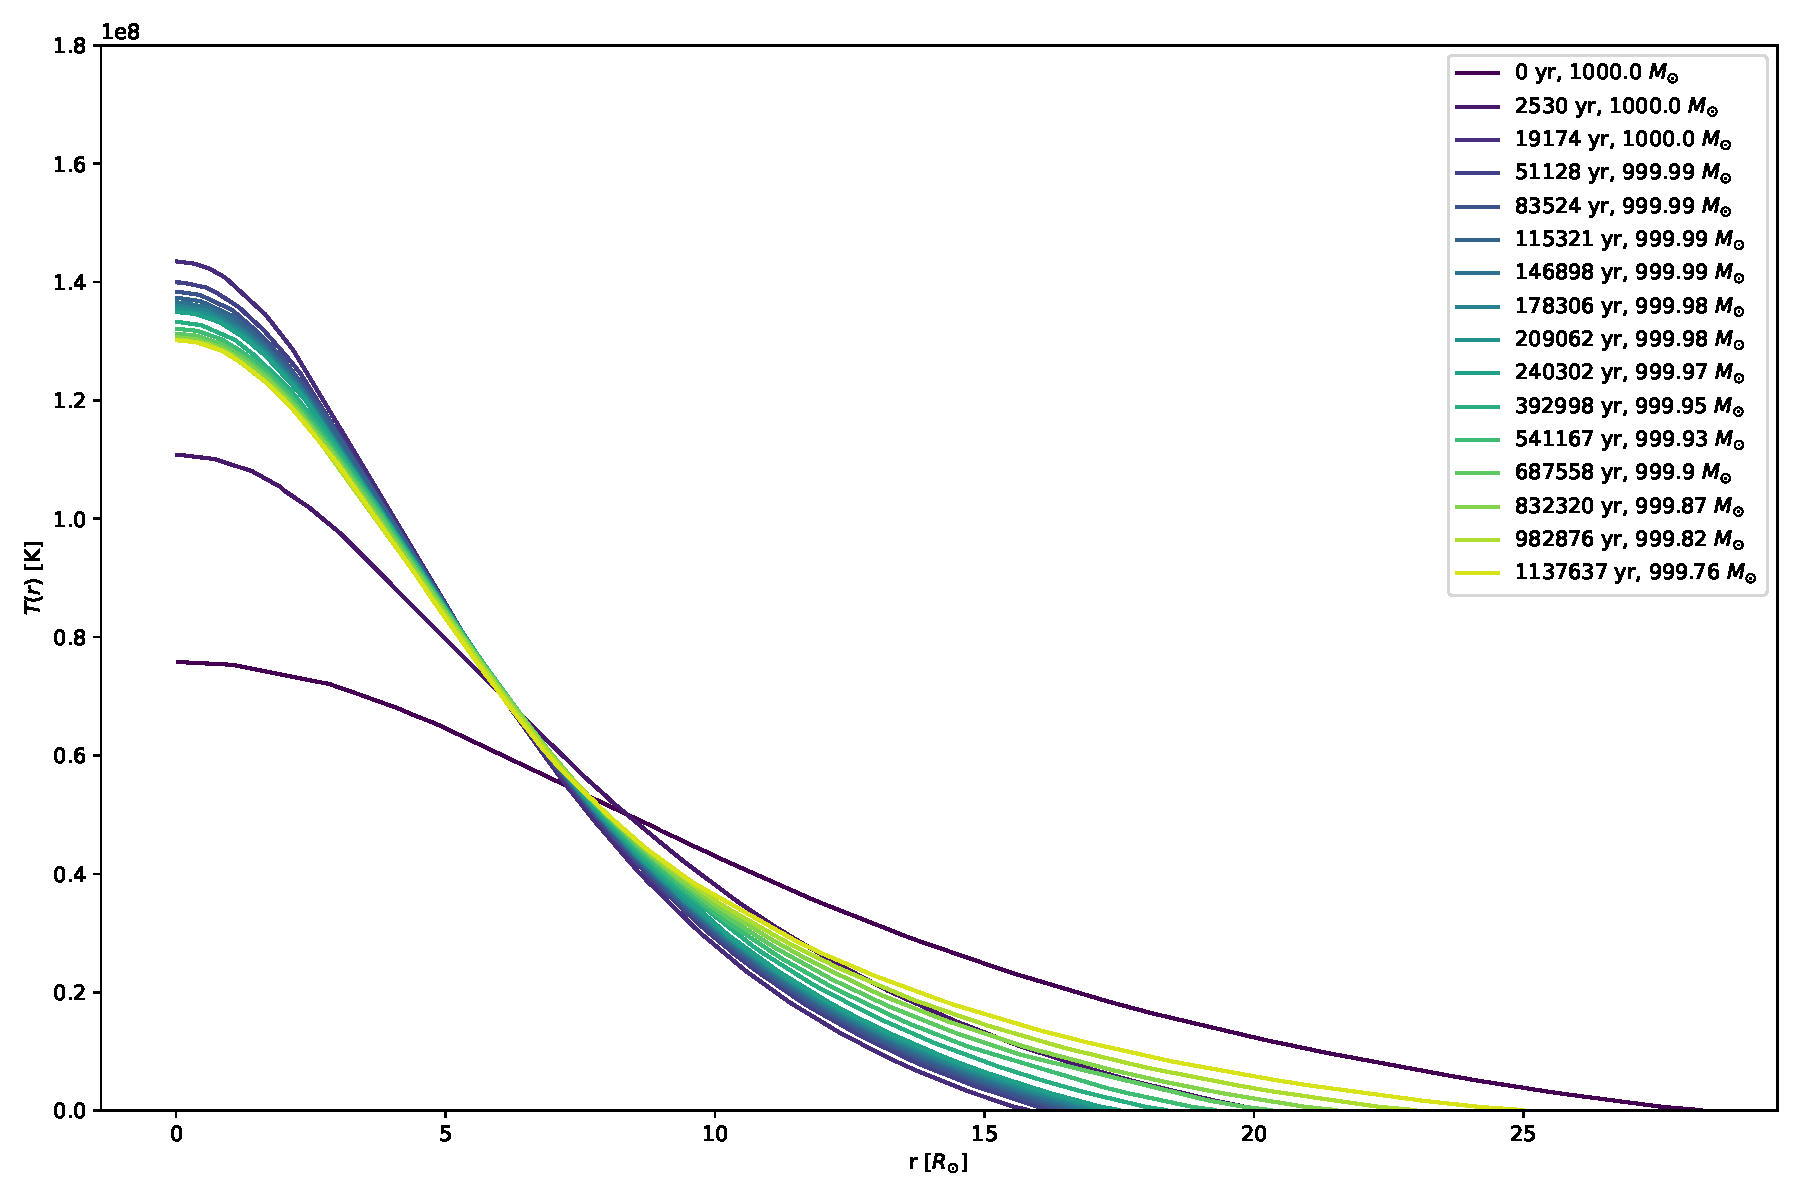
\includegraphics[width=0.49\textwidth]{T_profile_noDM.pdf}
        \caption{Radial temperature profiles for two 1000 $M_\odot$ Pop.~III stars, one with DM heating (left), and one without (right). For the left plot: $m_\chi = 10^{14}$ GeV and $\rho_\chi = 10^{16}$ GeV cm$^{-3}$.}
        \label{MESAtemp}
    \end{figure}
    \begin{figure}
        \centering
        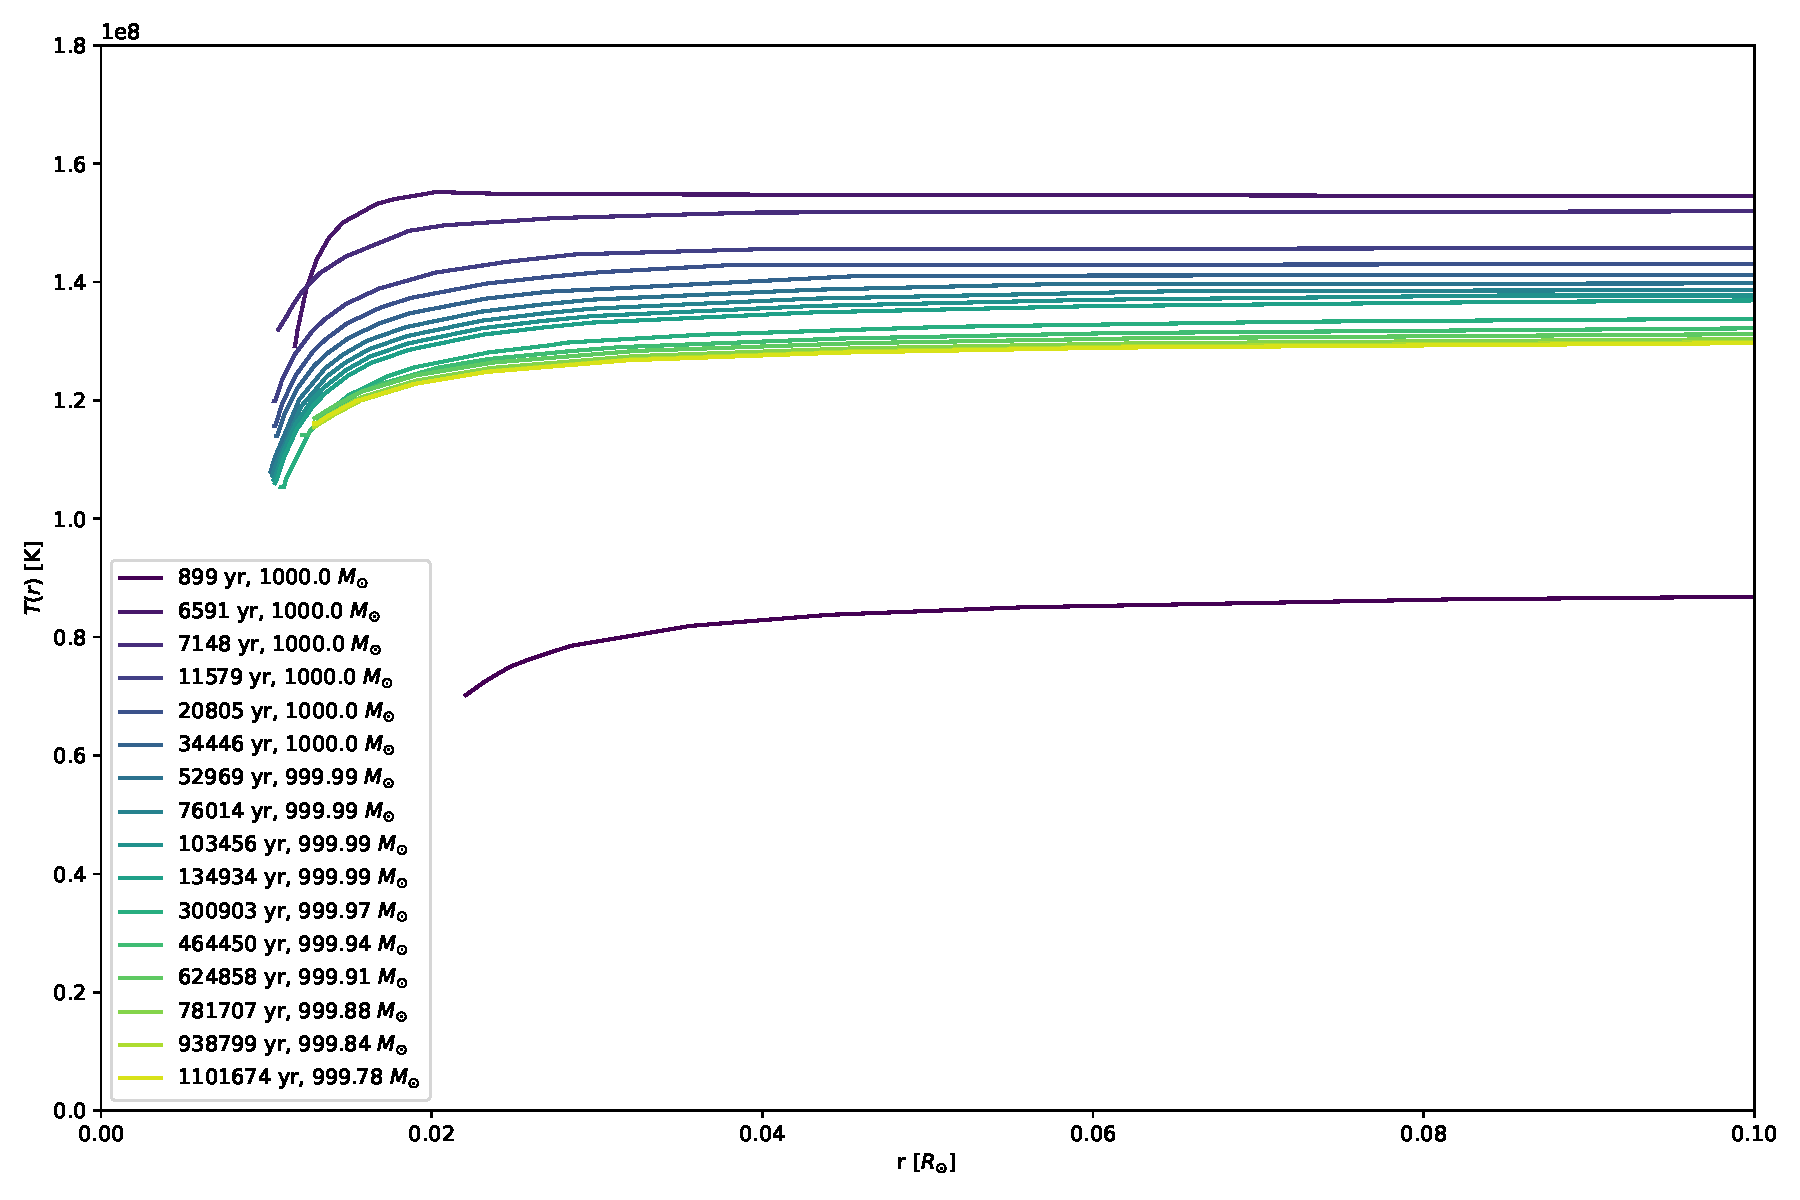
\includegraphics[trim={0 0.25cm 0 0.25cm},clip,width=1\textwidth]{Tcore.pdf}
        \caption{Same as the left plot in Fig.~\ref{MESAtemp} but zoomed in on the stellar core to show effects of DM heating. DM parameters: $m_\chi = 10^{14}$ GeV and $\rho_\chi = 10^{16}$ GeV cm$^{-3}$.}
    \end{figure}
    \begin{figure}
        \centering
        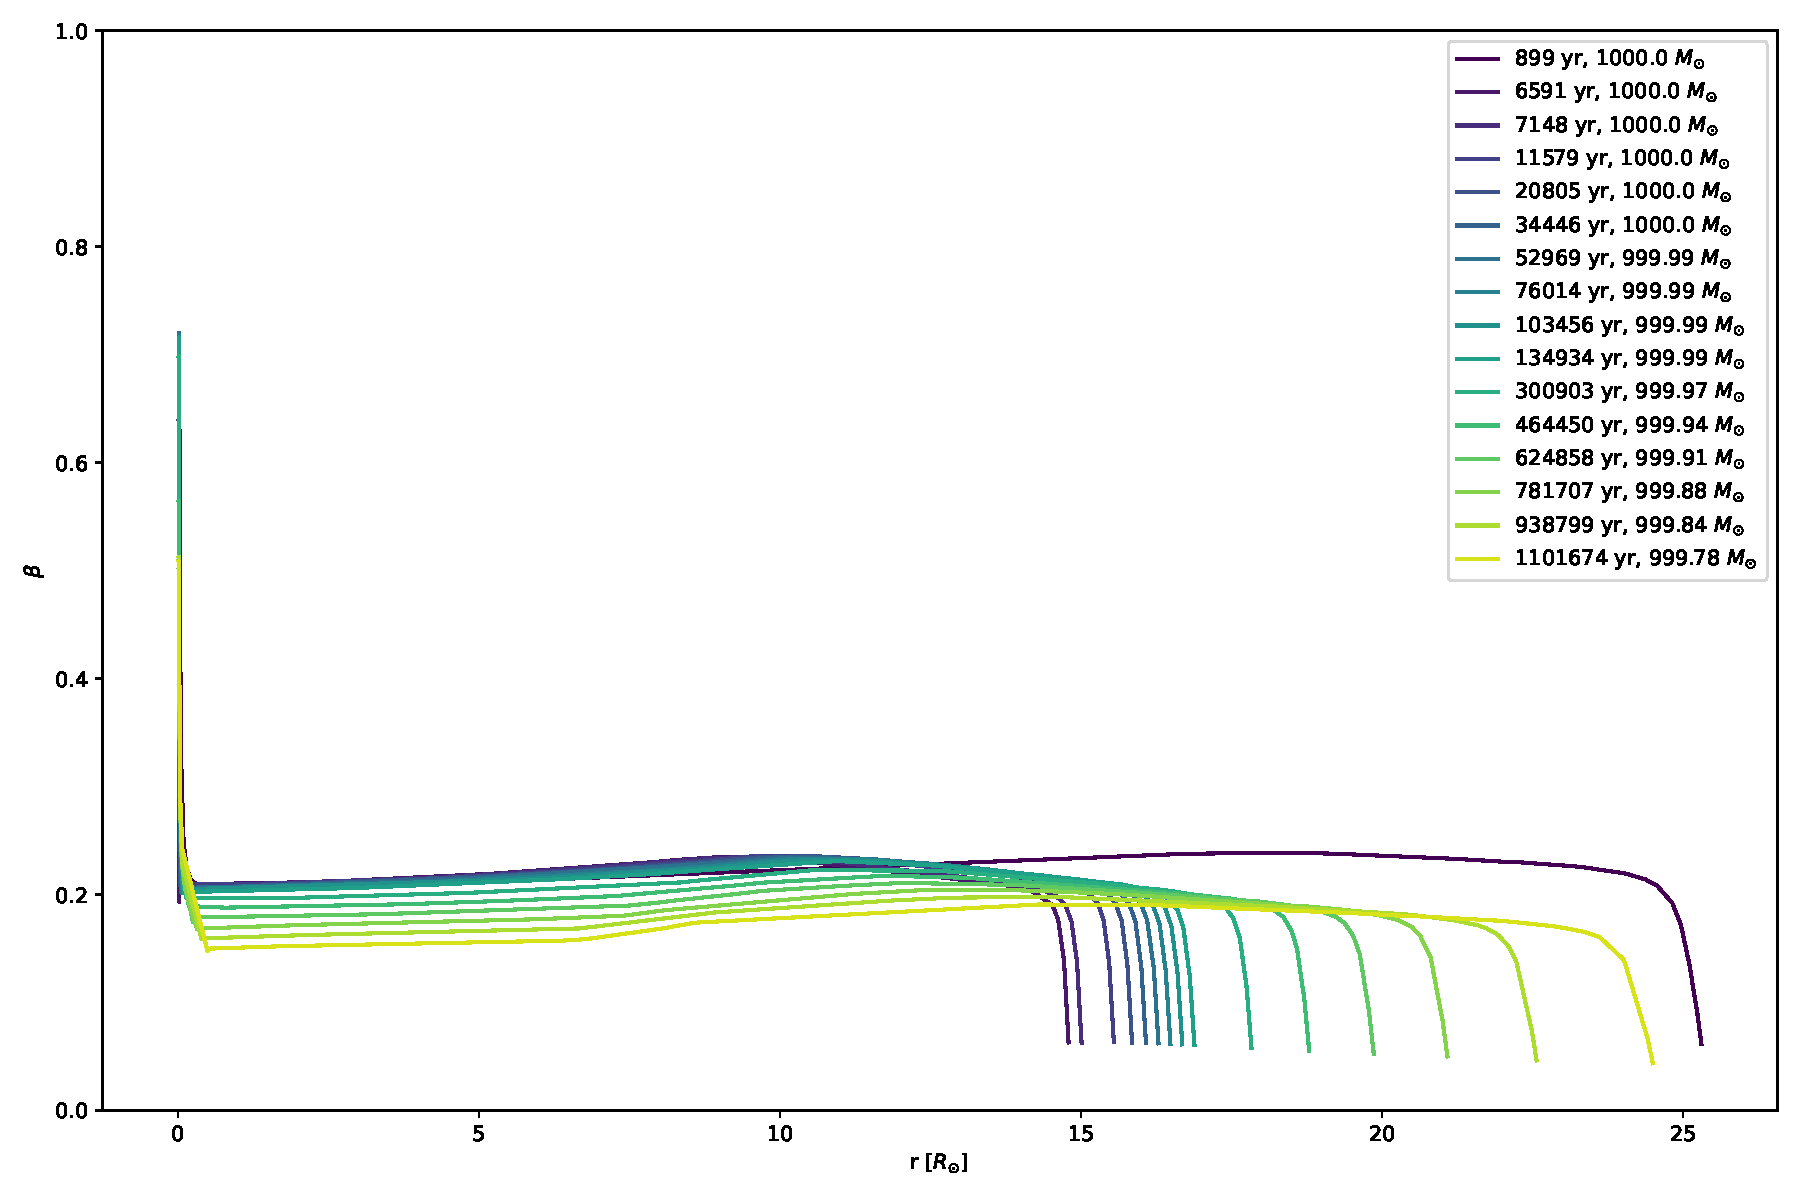
\includegraphics[width=0.49\textwidth]{beta_profile_DM.pdf}
        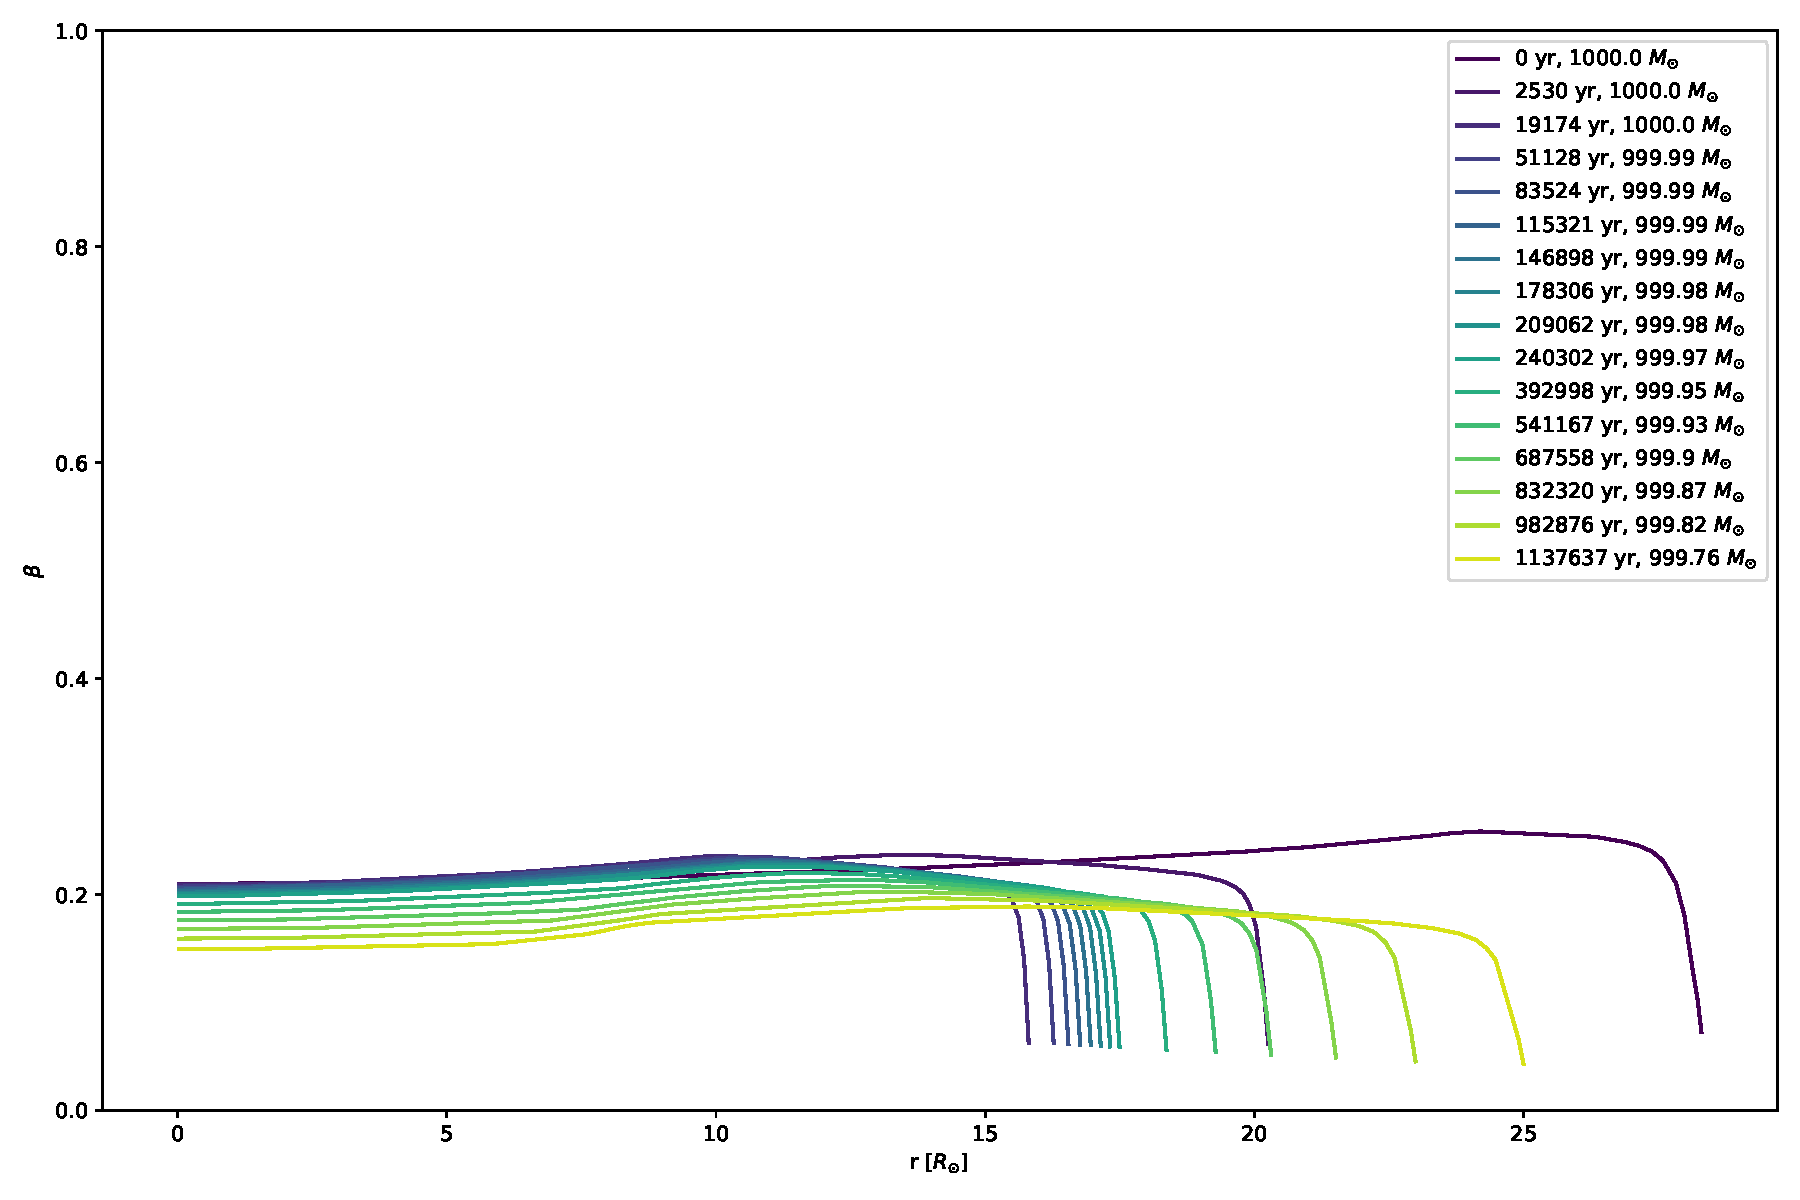
\includegraphics[width=0.49\textwidth]{beta_profile_noDM.pdf}
        \caption{Gas pressure to total pressure ratio for two 1000 $M_\odot$ Pop.~III stars, one with DM heating (left), and one without (right). For the left plot: $m_\chi = 10^{14}$ GeV and $\rho_\chi = 10^{16}$ GeV cm$^{-3}$.}
        \label{beta}
    \end{figure}
    \begin{figure}
        \centering
        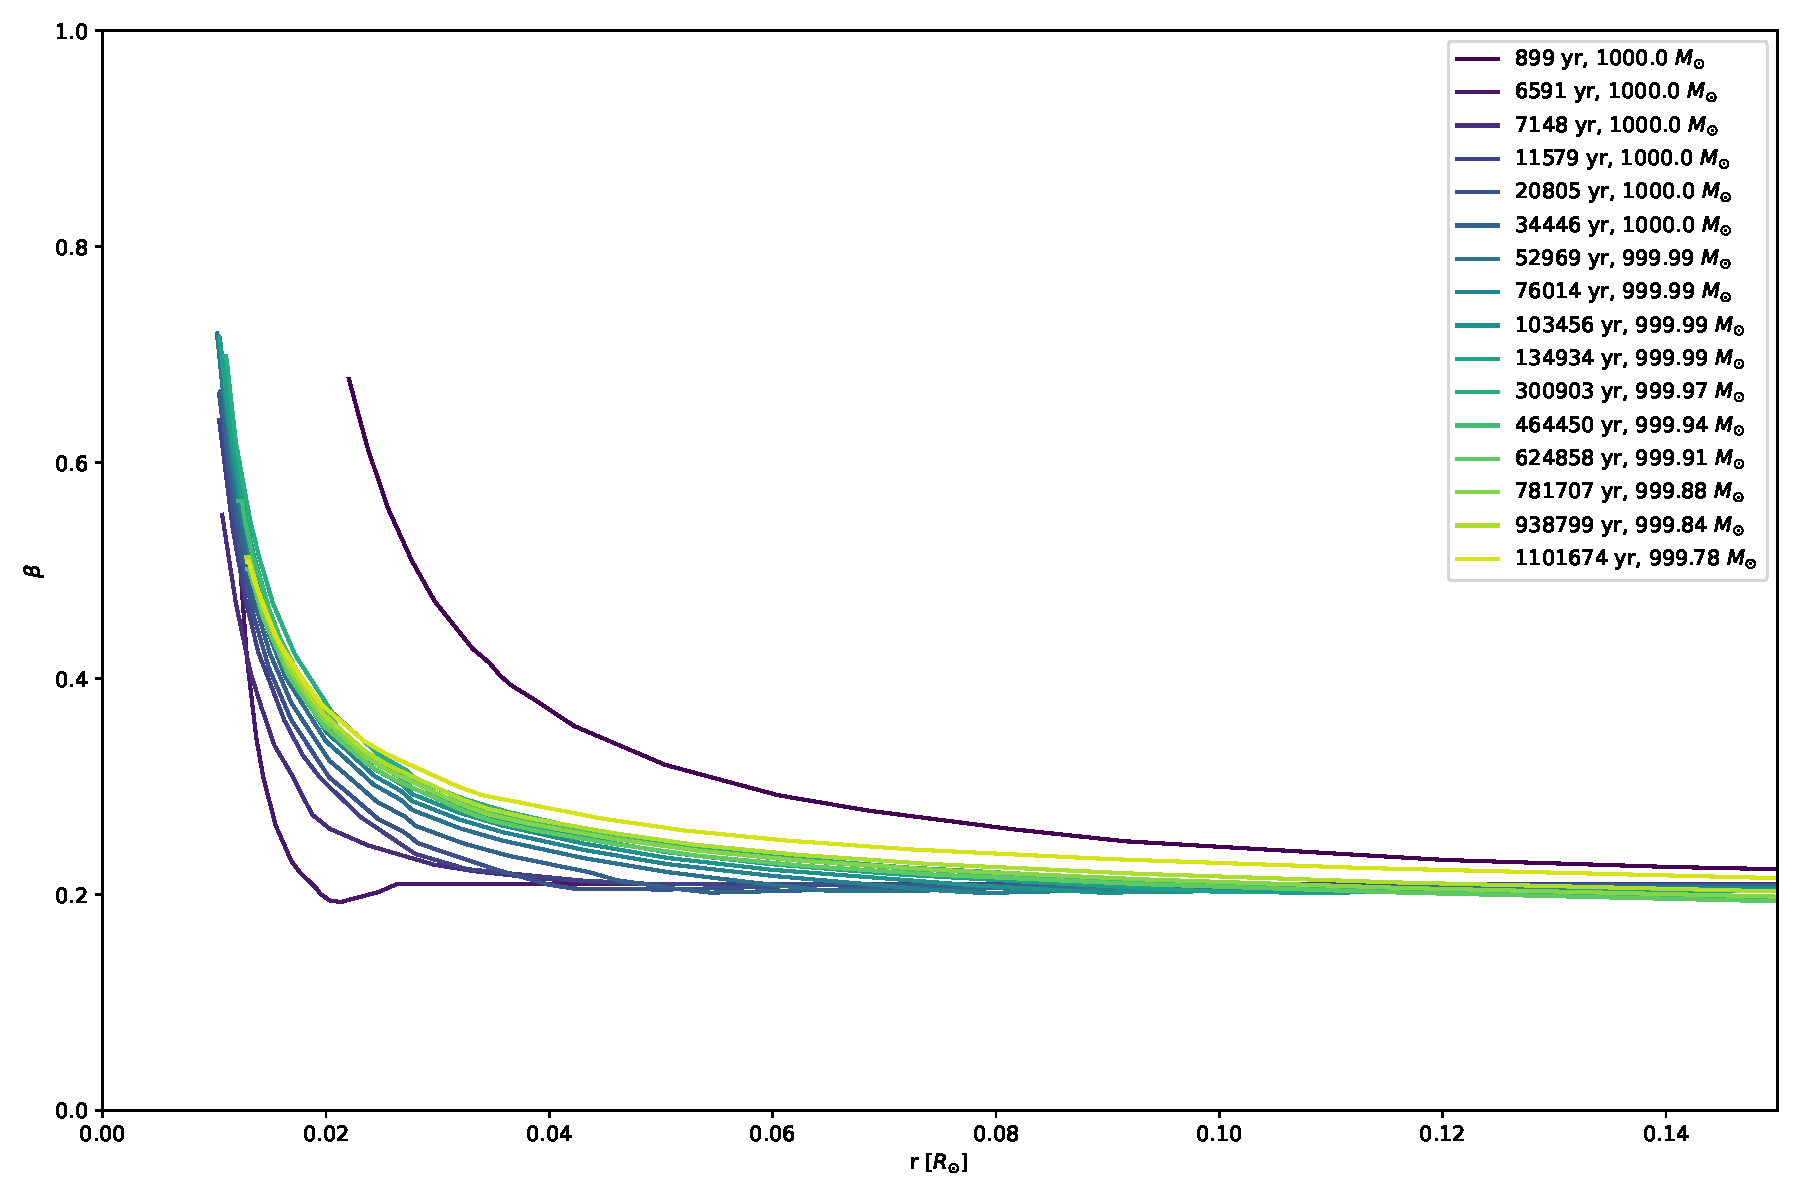
\includegraphics[trim={0 0.25cm 0 0.25cm},clip,width=1\textwidth]{beta_core_DM.pdf}
        \caption{Same as the left plot in Fig.~\ref{beta} but zoomed in on the stellar core to show effects of DM heating. DM parameters: $m_\chi = 10^{14}$ GeV and $\rho_\chi = 10^{16}$ GeV cm$^{-3}$.}
    \end{figure}
    \begin{figure}
        \centering
        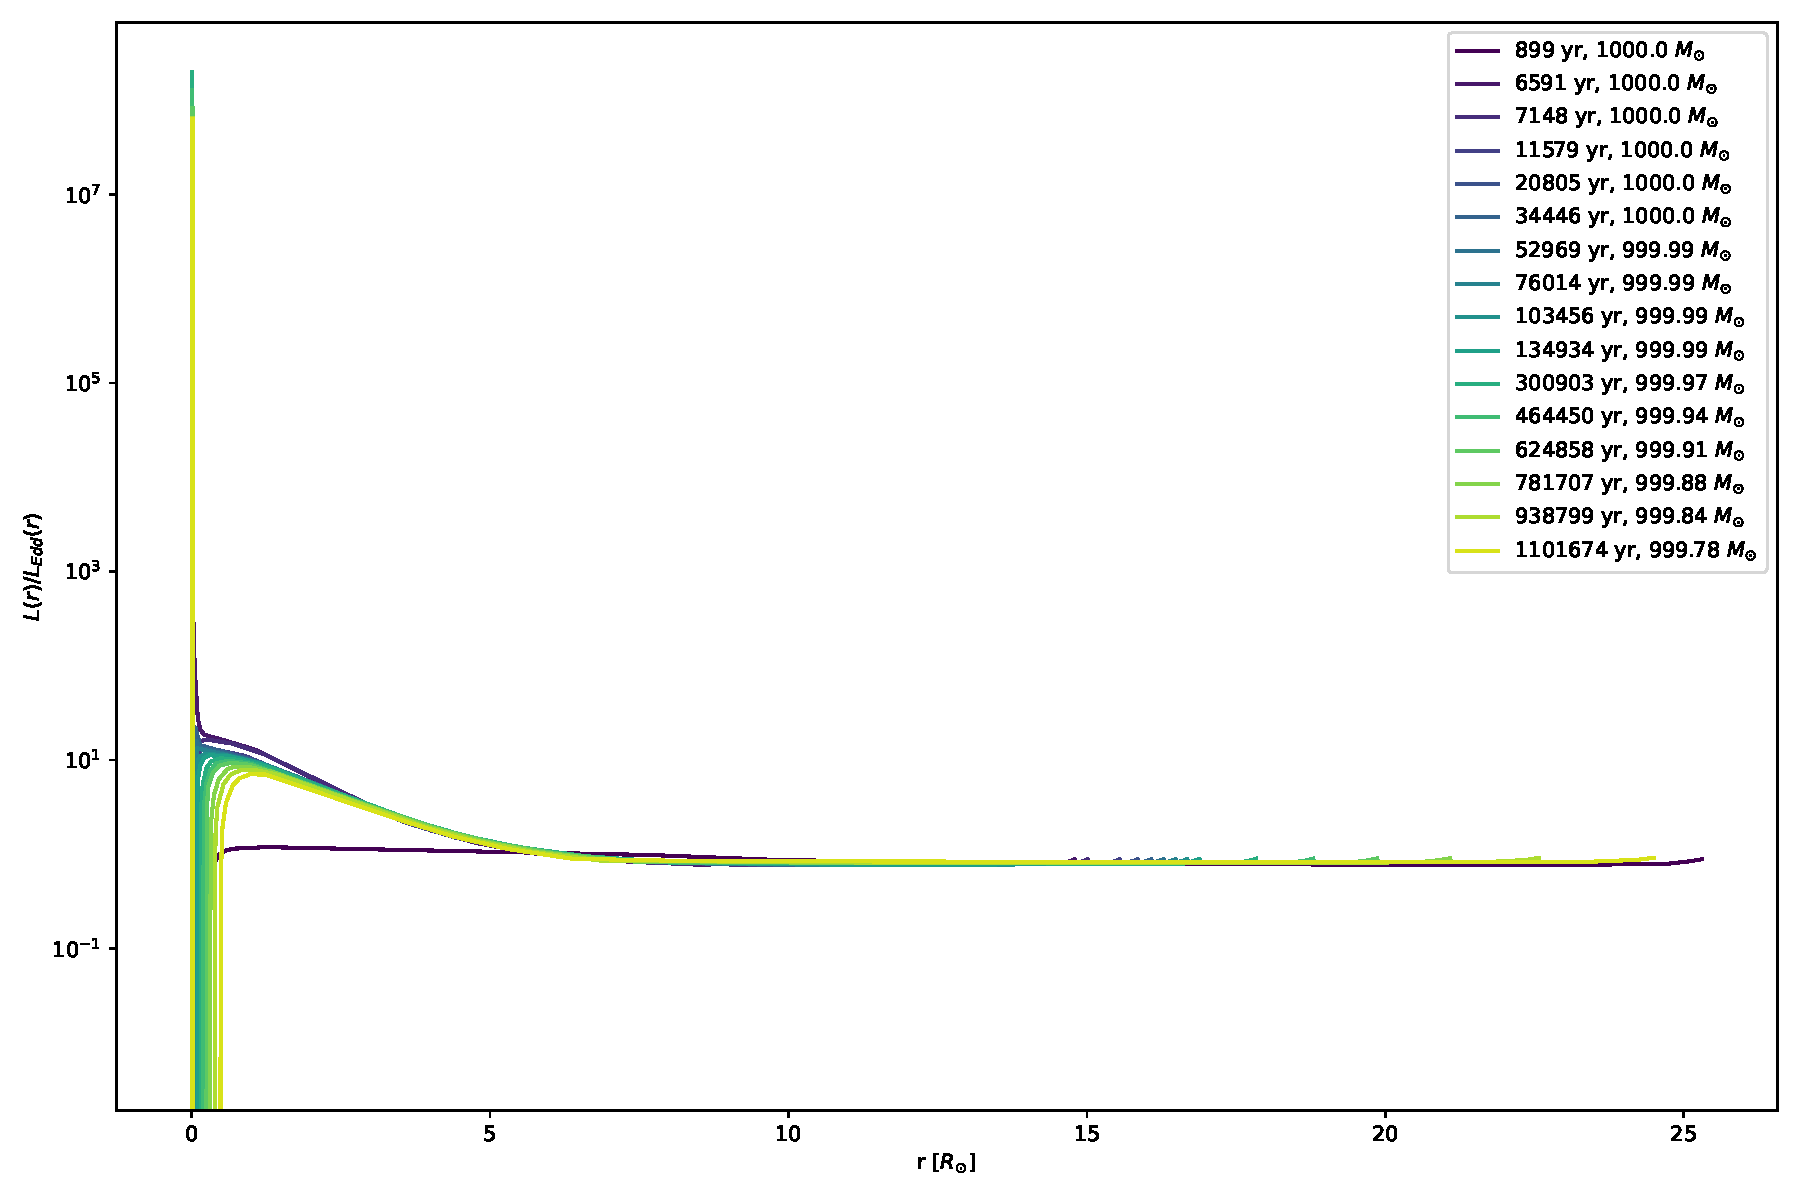
\includegraphics[trim={0 0.25cm 0 0.25cm},clip,width=0.8\textwidth]{Eddprof_DM.pdf}
        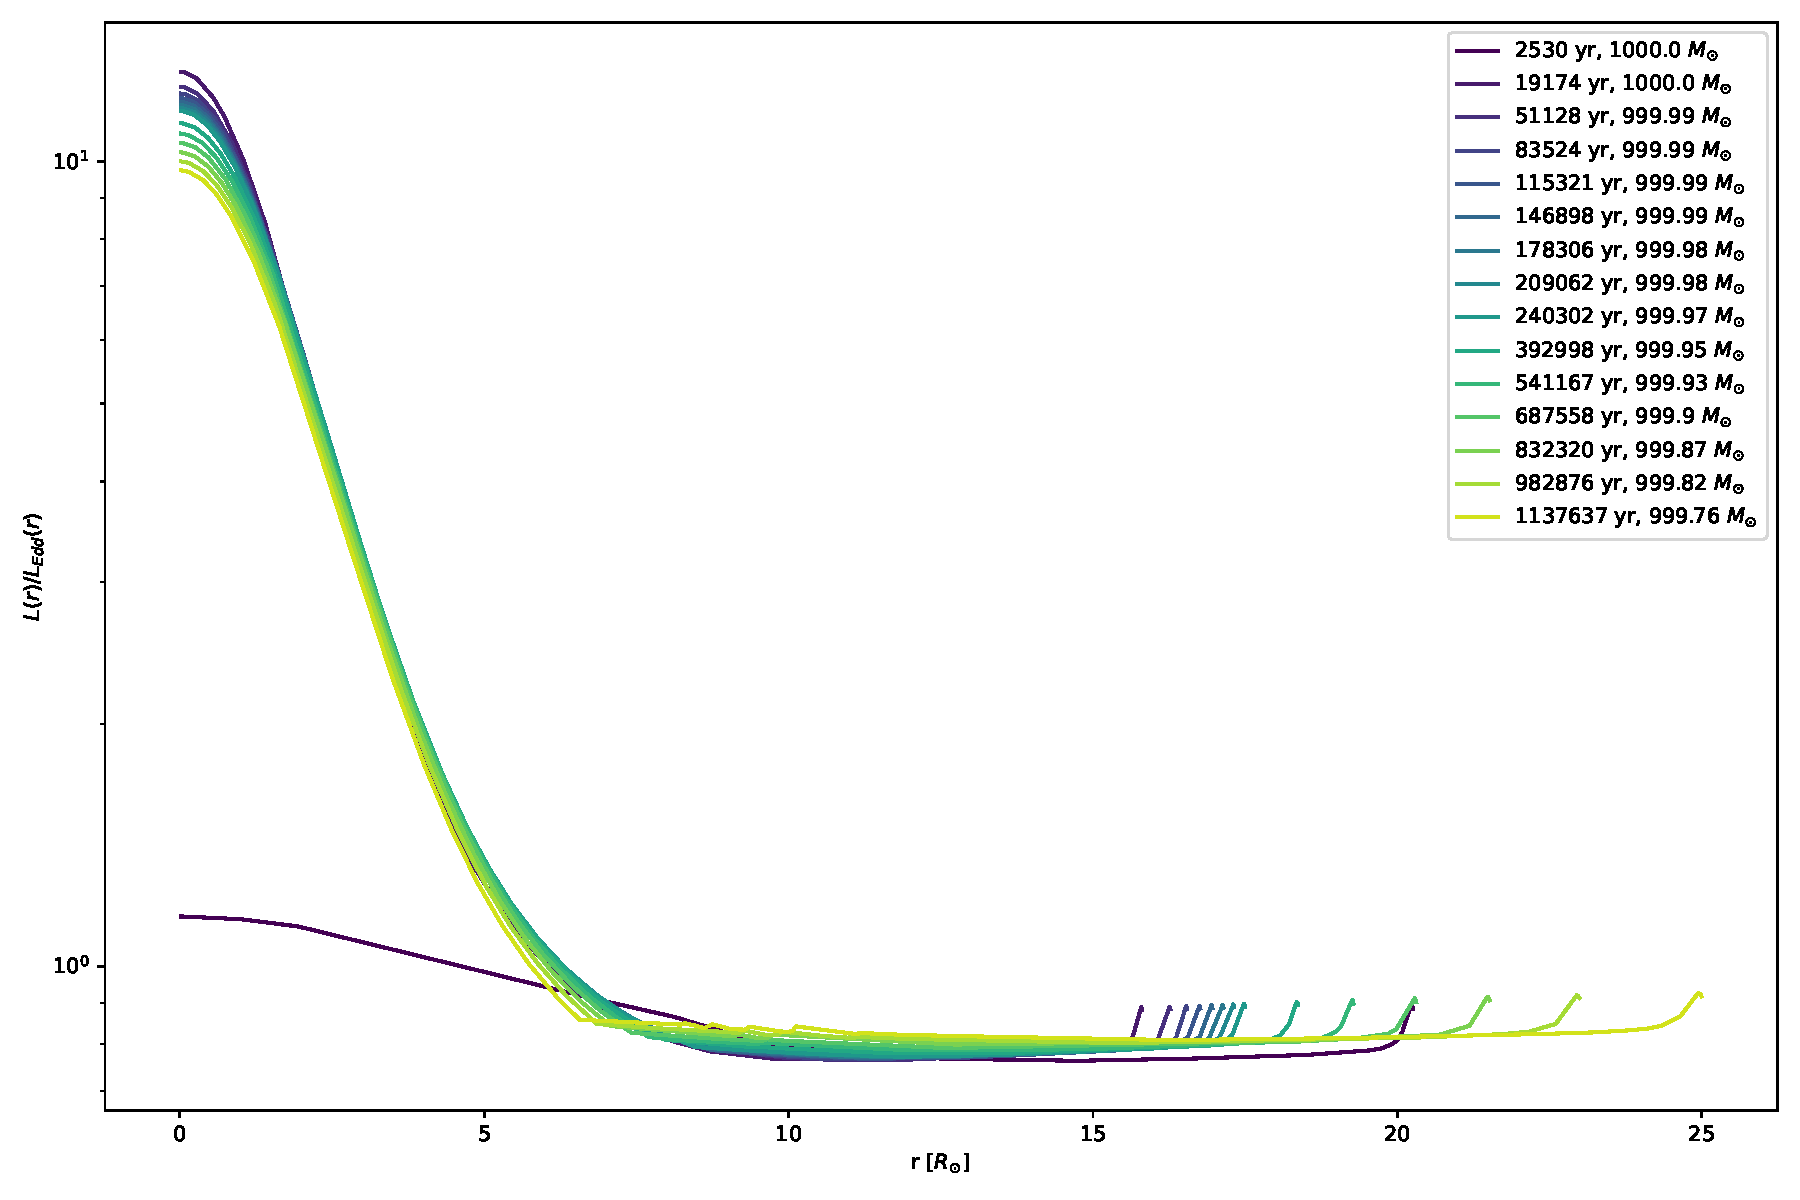
\includegraphics[trim={0 0.25cm 0 0.25cm},clip,width=0.8\textwidth]{Eddprof_noDM.pdf}
        \caption{Local Eddington ratio for two 1000 $M_\odot$ Pop.~III stars, one with DM heating (top), and one without (bottom). For the top plot: $m_\chi = 10^{14}$ GeV and $\rho_\chi = 10^{16}$ GeV cm$^{-3}$. Note the different scalings and the extreme Eddington ratio at the core of the DM heated star.}
        \label{eddplot}
    \end{figure}

    In this section I will consider an example of a DM heated Pop.~III star at the extreme end of my parameter space, a 1000 $M_\odot$ star, existing in an ambient DM density of $\rho_\chi = 10^{16}$ GeV cm$^{-3}$ and a DM mass of $m_\chi = 10^{14}$ GeV.
    I will compare this object against a standard Pop.~III star which I find matches closely with examples in the literature \cite{Windhorst:2019}.
    In terms of energy production, a DM heated Pop.~III star existing in these conditions should experience DM heating many orders greater than its nuclear heating.
    We find this to be true, with the total integrated \texttt{extra\_heat} to be $\sim 10^{55}$ erg s$^{-1}$ whereas the total luminosity of the non-DM heated star is $\sim 10^{41}$ erg s$^{-1}$.
    Despite this the stars still share many similarities and as stated before, I see no substantive super-Eddington winds.

    \begin{figure}
        \centering
        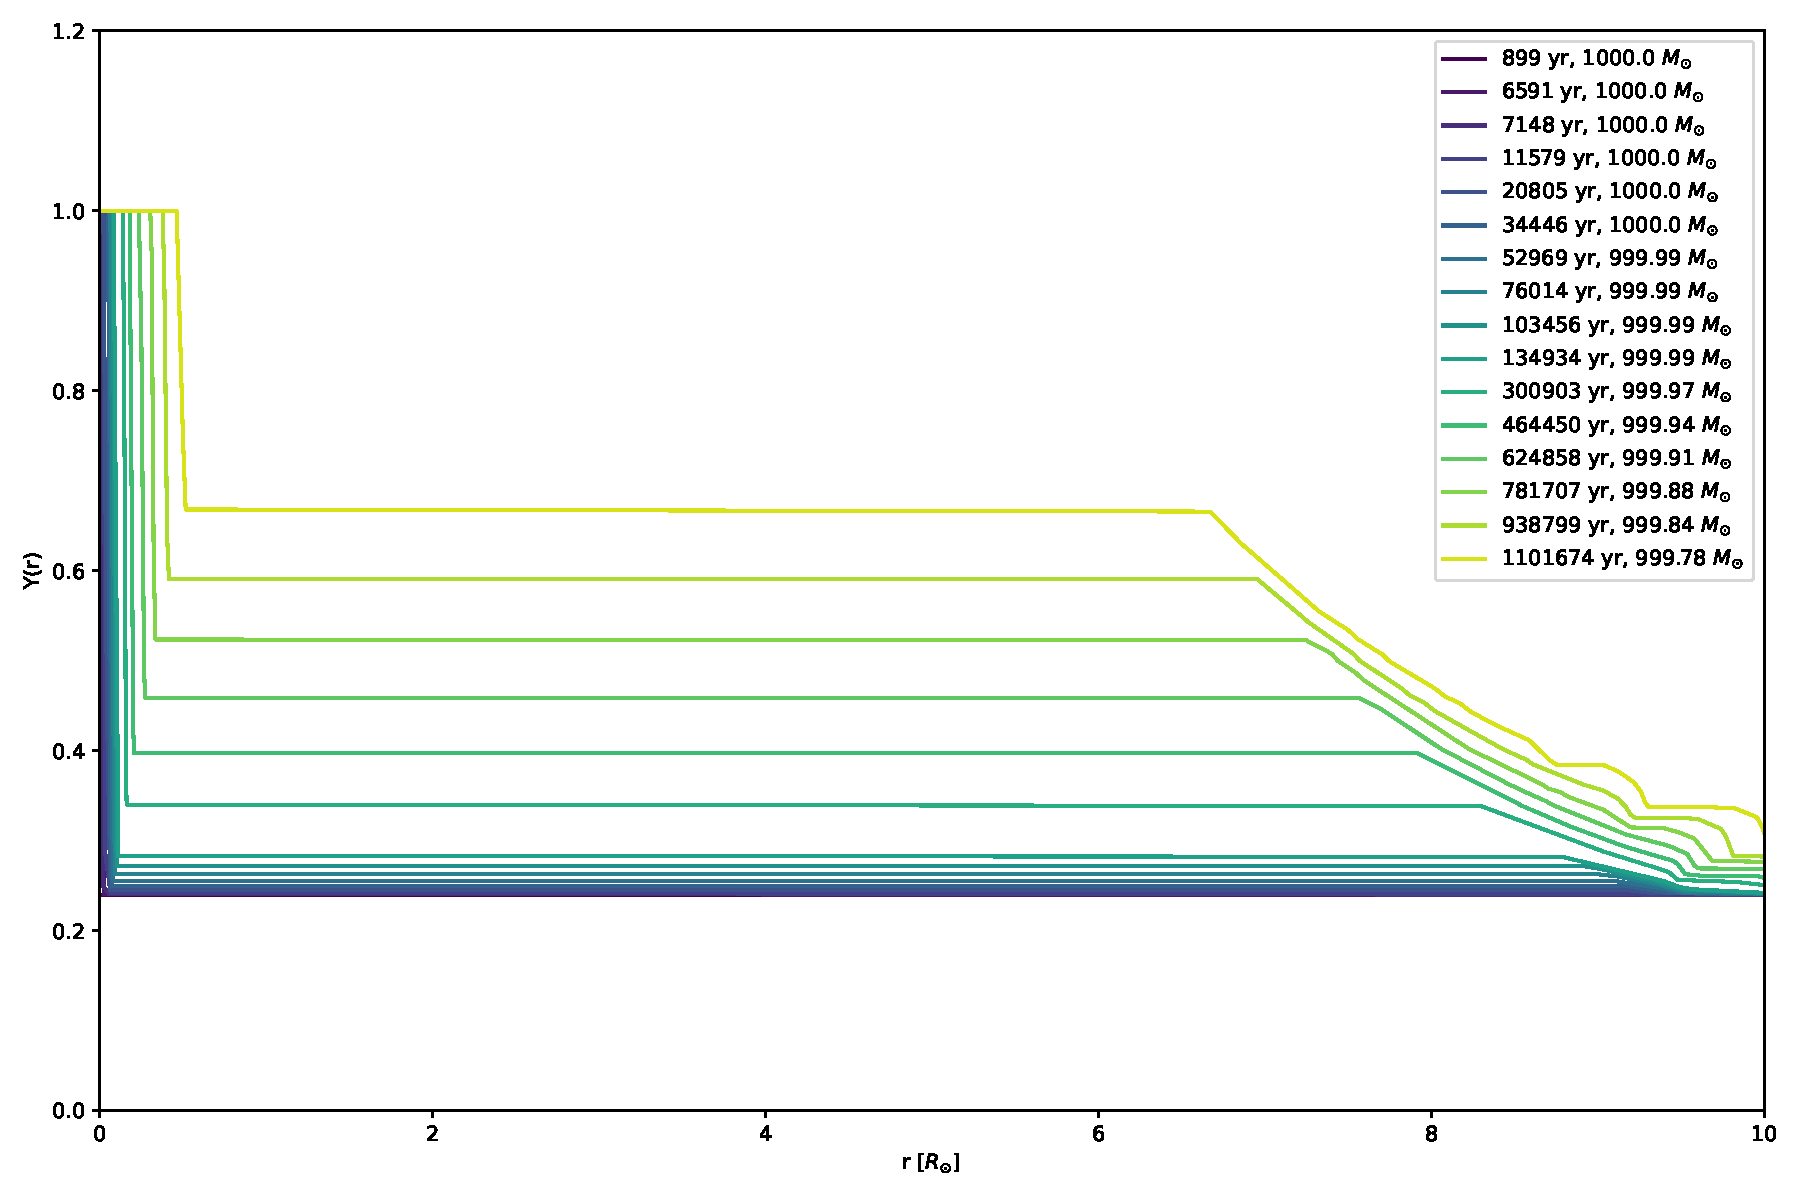
\includegraphics[width=0.8\textwidth]{Yfrac_DM.pdf}
        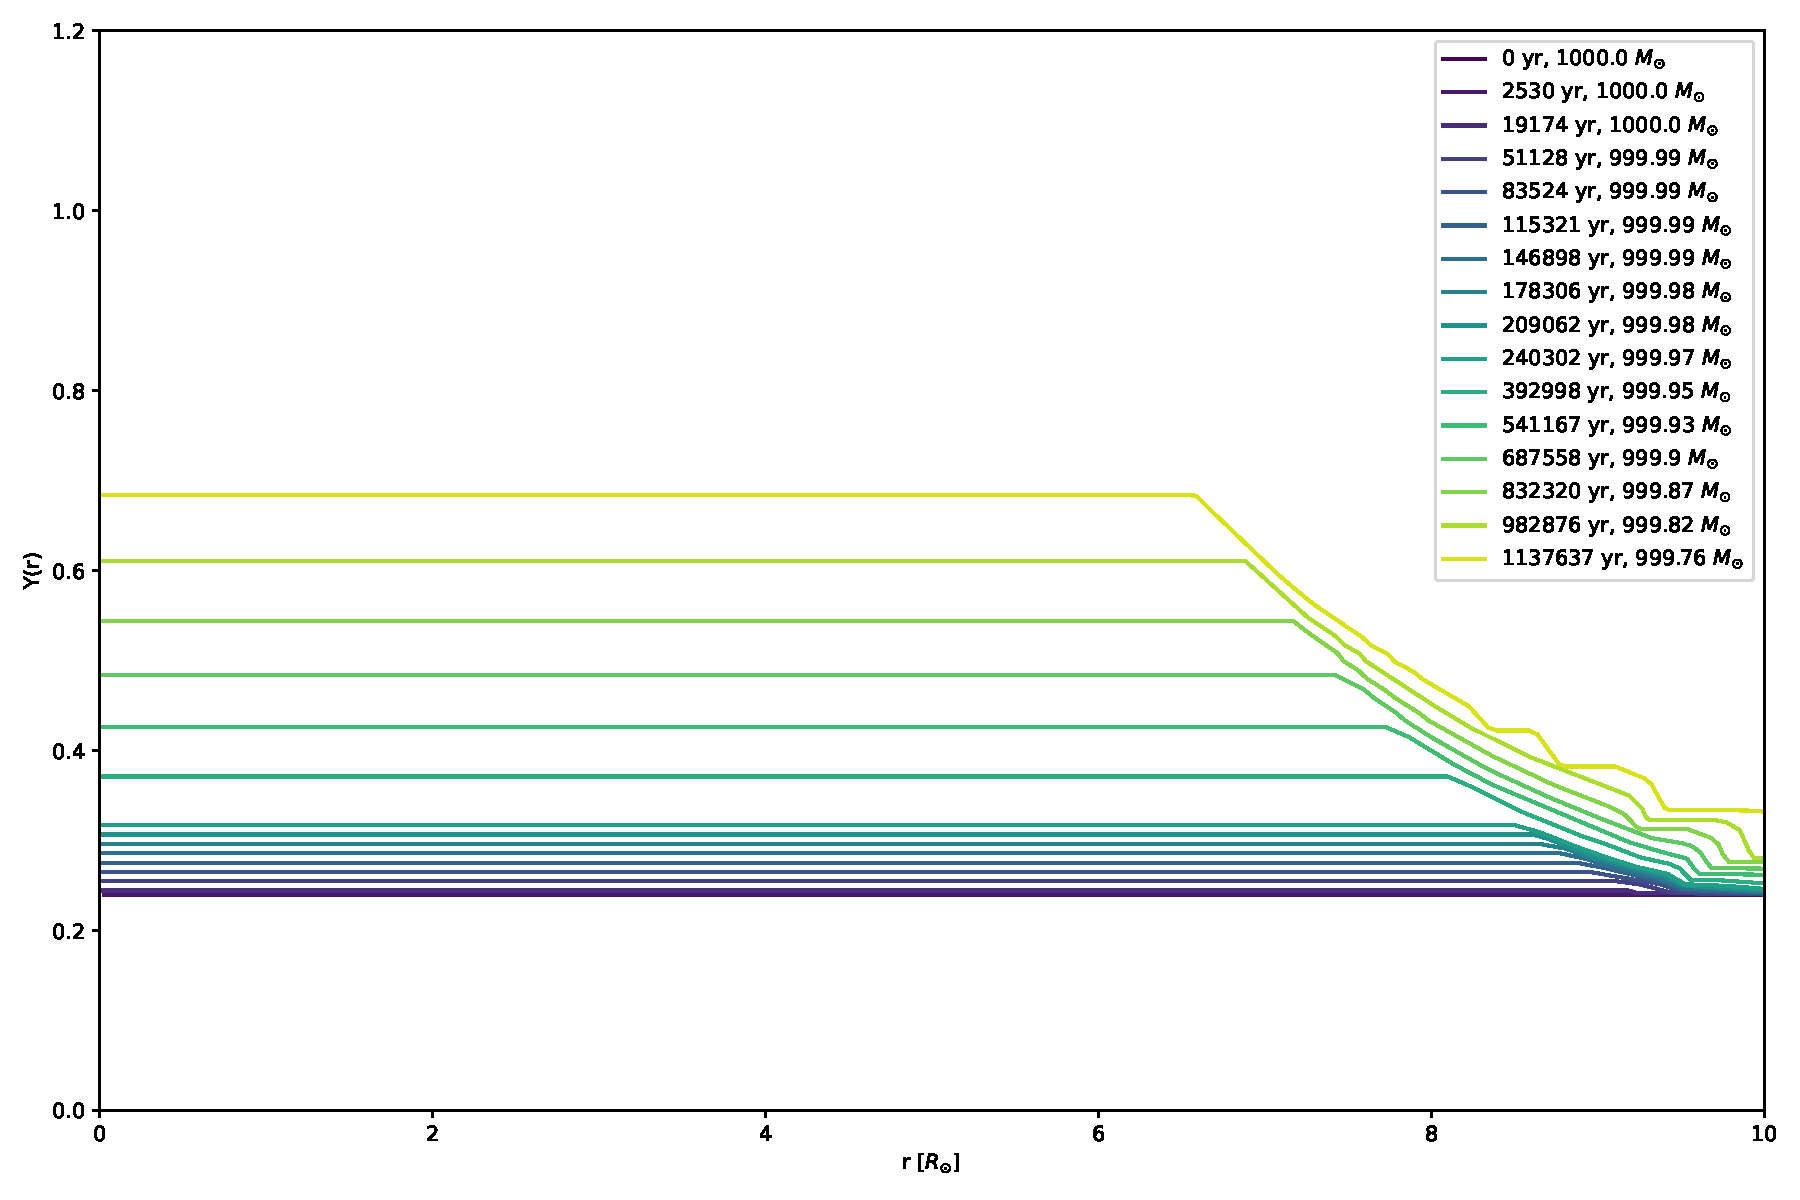
\includegraphics[width=0.8\textwidth]{Yfrac_noDM.pdf}
        \caption{Helium mass fraction for two 1000 $M_\odot$ Pop.~III stars, one with DM heating (top), and one without (bottom). For the top plot: $m_\chi = 10^{14}$ GeV and $\rho_\chi = 10^{16}$ GeV cm$^{-3}$.}
    \end{figure}

    The first feature of note is the radial temperature profile.
    Throughout the star we see nearly identical temperature values for both objects for the entirety of both their evolutions.
    However, at the core of the DM heated star we see a temperature inversion, where the temperature maxima sits at a distance of $\sim$ 0.02 $R_\odot$ from the center of the star.
    Central temperatures of the DM heated star are roughly $\sim 1.4$ times lower than non-DM heated star.

    Now turning our attention to modes of energy transport, we see that $\beta$, defined as the ratio of the gas pressure to the total pressure: $\beta = p_{gas} / p$, follows a similar pattern.
    Both stars have a constant values $\beta \approx 0.2$ throughout the star, until reaching the outer envelope where $\beta$ drops to zero.
    Again, the only difference between these two objects is at the core where we see values as high as $\sim 0.75$ in the DM heated star.
    This implies a convective inner core, and a strongly radiation dominated outer envelope.

    When considering the local Eddington factor (i.e.~$L_{rad}(r)/L_{Edd}(r)$) we again see similar behavior in the DM heated star.
    In the non-DM heated star the factor scales from $\sim$ 10 at the center to $\sim$ 0.5 for the majority of the star's radius.
    However, in the DM heated star we see a central Eddington factor of $\sim 10^7$. Again the DM heated star matches with the control Pop.~III star for the majority of radii.

    Finally, we move to He mass fraction, the most peculiar of the traits observed in the DM heated star.
    Starting as soon as the star passes ZAMS, we observe an inner region of 100\% helium composition in the core of the star.
    This region is on the order of $\sim$ 0.5 $M_\odot$ and grows throughout the star's lifetime.
    Accompanying this we see a reduction in the opacity of this region by a factor of $\sim$ 2.
    In the non-DM heated star we see a center Eddington fraction of $\sim$ 10, which quickly falls to a constant $\sim 0.2$ throughout the rest of the star.

    It is important to note that while this is the most extreme example of DM heating, these peculiarities in the models can be observed anytime the DM heating is significant as compared to nuclear heating.
    Furthermore, while I have optimized these models using inlist parameters to best represent Pop.~III stars, the same behaviors are observed while using default \texttt{MESA} inlists.
    That is to say, if the models are able to converge and run to completion we see the same phenomenon.
\end{section}



\begin{section}{Building Dark Stars Using Only Capture}
    In the standard model of Pop.~III formation, protostars begin to coalesce and undergo collapse as governed by the virial theorem inside Dark matter halos of up to $10^6$ M$_{\odot}$ \cite{Freese:2016dark}.
    These are often called minihalos, in contrast to the galactic DM halos of our current epoch.
    Material will continue to accrete as local gas infalls until the core of the protostar reaches a critical temperature of roughly $\sim10^8$ K when hydrogen burning begins.
    In the simplest picture we can assume Pop.~III stars form at the center of their host minihalo.
    Here, the volume that the star occupies will overlap with the highest Dark matter densities at the center of the halo, allowing for capture rates and subsequently, heating rates to be high enough to alter the evolutionary course of the star.
    This process will be dictated by local Dark matter densities, the DM-nucleon cross section, and DM particle mass.
    Notably, significant Dark matter heating opens up the possibility of an entirely new stellar phase driven entirely by Dark matter annihilation called a dark star.

    While modeling the effects of adiabatic contraction (AC), another method by which DM may heat a star, it has been shown that the beginning of nuclear burning in proto-Pop.~III stars can be prevented entirely if heating from AC is significant enough to form a dark star.
    Moreover, during the dark star phase, mass can continue to accrete onto the star so long as the DM reservoir from which AC draws does not run out.
    In work performed with \texttt{MESA}'s \texttt{run\_star\_extras.f} routine in a similar fashion to my own, has shown that it may be possible to form dark stars with masses up to $10^6 M_{\odot}$ and the subsequent stars are significantly hotter, brighter, and radially smaller then predicted by previous work \cite{Rindler-Daller:2015} \cite{Rindler-Daller:2020}.
    \begin{figure}
        \centering
        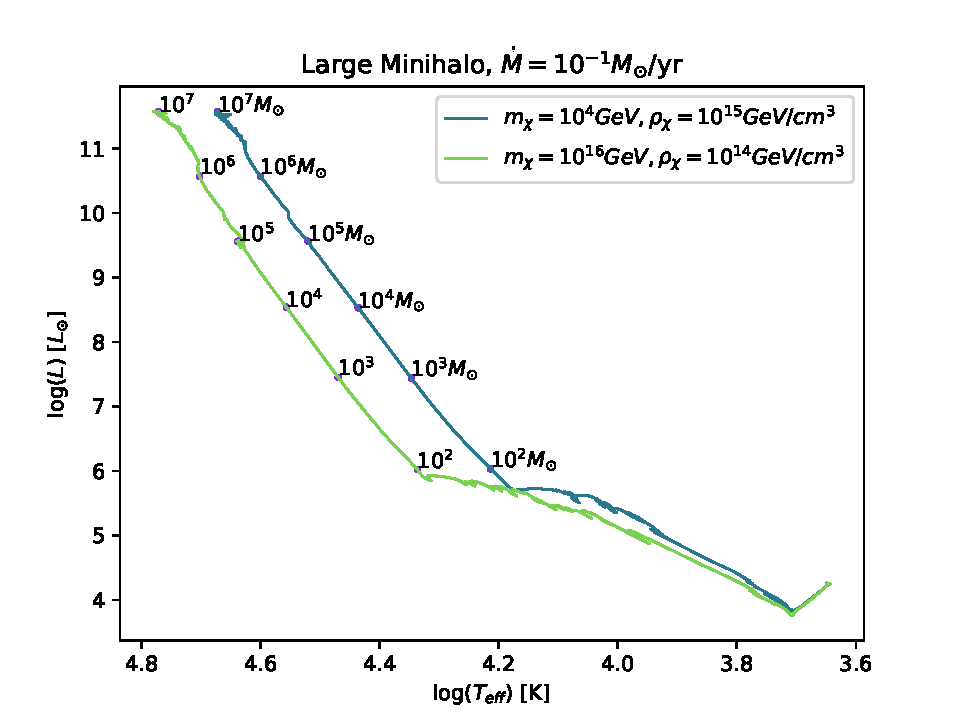
\includegraphics[trim={0 0.2cm 0 0.6cm},clip,width=0.8\textwidth]{hr.pdf}
        \caption{Evolutionary tracks of Pop.~III stars when considering heating from captured DM. Considering two different DM masses and DM densities. Stars continue to accrete mass as long as it is supplied by the surrounding halo.}
    \end{figure}

    For the work in this section, I closely mimic the conditions put forward in \cite{Rindler-Daller:2015} with the notable difference of considering heating from DM capture instead of that from AC.
    I start with the same initial central densities and temperatures from \cite{Rindler-Daller:2020}(who calculates them under the assumption of a $N=3/2$ polytrope) and I take proto-Pop.~III stars forming at $10 M_{\odot}$ and then accrete mass from the surrounding large minihalo at a rate of $\dot{M} = 10^{-1} M_{\odot}/$yr as long as the star is able.
    I find that, for high enough DM densities (i.e.~$10^{15}$ GeV/cm$^3$), heating from DM capture is significant enough to dominate over nuclear energy production and form a dark star-like object.
    The distinguishing factor between these objects and dark stars is the presence of minimal nuclear burning, which occurs out of necessity since DM heating from capture is dependent on the density of the object doing the capturing.
    During the initial collapse of the proto-star, DM heating won't `kick in' until the core of the proto-star has reached high enough temperatures to begin hydrogen burning.
    However, once this density is achieved DM heating from capture will almost immediately outstrip nuclear heating.
    Moreover, I find the same phenomena of super massive dark star formation as in \cite{Rindler-Daller:2015}: at appropriately high DM densities stars powered by captured DM will continue to accrete mass, until potentially even $10^7 M_{\odot}$.

    The key difference between these models and the previous sections is the presence of continuing cold accretion.
    This accretion allows the star to stay well below the Eddington limit for its mass.
    Further work needs to be undertaken to compare these models with the previous sections to understand exactly how and why they diverge in behavior.

    If these models represent something truly physical, objects of this size and brightness would be ideal candidates for observation by the soon to be launched James Webb Space Telescope.
    Not only would dark stars represent a fascinating new astrophysical object to study, but they could serve as cosmological standard candles, instruments for probing the characteristics of Dark matter, or precursors to intermediate or supermassive black holes.

    As interesting as these results are, I should stress that at time of writing I have only begun to collect data with this new \texttt{MESA} methodology and there is still much to be done in terms of testing. 
    Moreover, the numerical techniques outlined in this work are still in their infancy and have yet to be fully validated.
\end{section}



\begin{section}{Future Work}
    Further work on studying DM heating in \texttt{MESA} clearly needs to be undertaken.
    As DM direct detection experiments approach the neutrino floor, particle physicists and astronomers alike must find new and creative methods to bound the DM parameter space.
    Using objects like Pop.~III stars as astrophysical laboratories may very well be the key to discovering DM.
    Beyond further testing and validation of the methods outlined in this paper, work should proceed on the incorporation of equilibration timescales, DM evaporation, and multicomponent capture (i.e.~H and He) in my existing code base.
    All of this should be incorporated into an open source \texttt{MESA} module to allow others to conduct further experimentation.
    Finally, these capture routines should be combined with existing extended AC code, and ultimately AC, in order to get a full picture of the influence DM may have on the first stars.
\end{section}



\begin{acknowledgments}
    I would like to thank both Caleb Levy and Jillian Paulin who have spent innumerable hours of their lives helping me debug code.
    They both are incredibly capable researchers, and are always eager to help.
    I count myself lucky to have them as colleagues.
    Finally, I want to thank my advisor, Cosmin Ilie, for all the opportunities he as provided me as a researcher.
\end{acknowledgments}

\bibliographystyle{JHEP}
\bibliography{RefsDM}



\end{document}
